%************************************************
\chapter{The LUX Detector}

\label{ch:lux} % $\mathbb{ZNR}$
%************************************************

%\begin{flushright}{\slshape    
%   I'm the hottest in the street \\
%   Know you prolly heard of me } \\ \medskip
%    --- {Cardi B, \textit{Bodak Yellow}, 2017}
%\end{flushright}



\section{LUX Overview}
The \ac{LUX} detector was an ultra-low background dual phase liquid xenon \ac{TPC} that set world-leading limits on \ac{WIMP} interactions.
 
\ac{LUX} began underground commissioning in July 2012, moving to the 4850 level (4300~m.w.e) of \ac{SURF} in Lead, South Dakota.  The \ac{LUX} Collaboration's first \ac{WIMP} search exposure was for a period of 85.3 live-days, acquired between April 2013 and August 2013. This period of time is referred to as Run03, and the \ac{WIMP} result is referred to as WS2013. The detector then underwent a grid conditioning campaign to improve voltage capabilities, followed by a series of extensive calibrations to characterize the new operating conditions. The detector then ran for a period of 332 live-days from September 2014 to May 2016 (Run04, WS2014-2016), ending with decommissioning in September 2016. Run03 and Run04 had distinct operating conditions and calibrations. The \ac{LIP} search in Chapter~\ref{ch:lips} was carried out using Run03 data, and the calibrations in the latter half of this chapter describe the detector conditions as they were in Run03. 

\section{Internal Components}
The major internal components of \ac{LUX} are shown in Figure~\ref{fig:lux1}. The active volume of \ac{LUX} was composed of 300~kg of liquid xenon, instrumented with two arrays of Hamamatsu R8778 \ac{VUV}-sensitive \ac{PMT}s viewing the liquid region from the top and bottom. Both arrays were composed of 61 \ac{PMT}s that detected S1 and S2 photons from particle interactions in the active liquid volume, and were held in place by copper mounting blocks. The \ac{PMT}s were tightly packed in a hexagonal formation to maximize light collection. The xenon-facing surfaces the of copper \ac{PMT} mounting blocks were covered with \ac{PTFE} tri-foils to reflect the 178~nm light, since copper is a poor reflector of \ac{VUV} light. 

The active region was defined by a series of strung wire or mesh grids: the cathode grid was at the bottom of the detector, and the gate grid was 48.3~cm above the cathode when cold. These two grids formed the drift field, which was \~180~kV/cm during Run03. The region between the cathode and gate grids is known as the drift region, it is where particle interactions take place. The anode mesh plane was 1~cm above the gate grid, and the xenon liquid level was held constant between these two electrodes by a spillover weir. The anode and gate form the extraction region of the experiment, where electrons are extracted across the liquid-gas boundary and undergo proportional scintillation to form S2. There are two additional grids, the top and bottom grids, which are placed 2~cm from the top and bottom \ac{PMT} arrays to insulate the \ac{PMT}s from the high fields produced by the other grids. The top and bottom grids were held at approximately the same voltage applied to the \ac{PMT}s. All electrodes were 88\%-99\% optically transparent at normal incidence, and made of stainless steel 316.

\begin{figure}[htbp]
\begin{center}
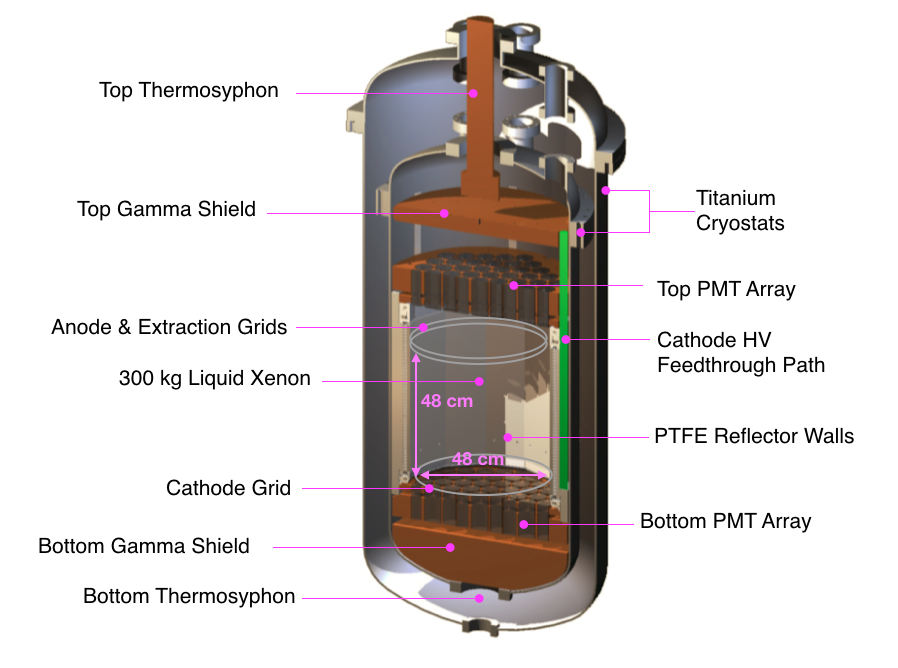
\includegraphics[width=\textwidth]{figures/lux/lux_inner1.png}
\caption{Major components and dimensions of the \acs{LUX} detector. Figure from \cite{LUXDetectorPaper}. }
\label{fig:lux1}
\end{center}
\end{figure}


The insides of the detector walls were lined with 12 \ac{PTFE} panels, which made the exact detector geometry a dodecagonal prism with flat faces, instead of a perfect cylinder with one rounded face. Immediately behind the \ac{PTFE} were 48 copper field-shaping ``rings'' (dodecagons). The rings were vertically separated by 1~cm, and the gate-to-cathode voltage was graded evenly over the rings by a resistor chain connecting the rings. 

Below and above the \ac{PMT} mounting blocks were two large solid copper domes which acted as gamma shields and also functioned as thermal mass that aided in keeping the detector temperature stable. The bottom dome also acted as a heat exchanger to quickly re-thermalize incoming xenon gas (from the circulation system) as it entered the liquid region. The bottom dome also minimized the volume filled with non-active liquid xenon. See Figure~\ref{fig:lux2} for details about the field-shaping rings and copper shields.

\begin{figure}[htbp]
\begin{center}
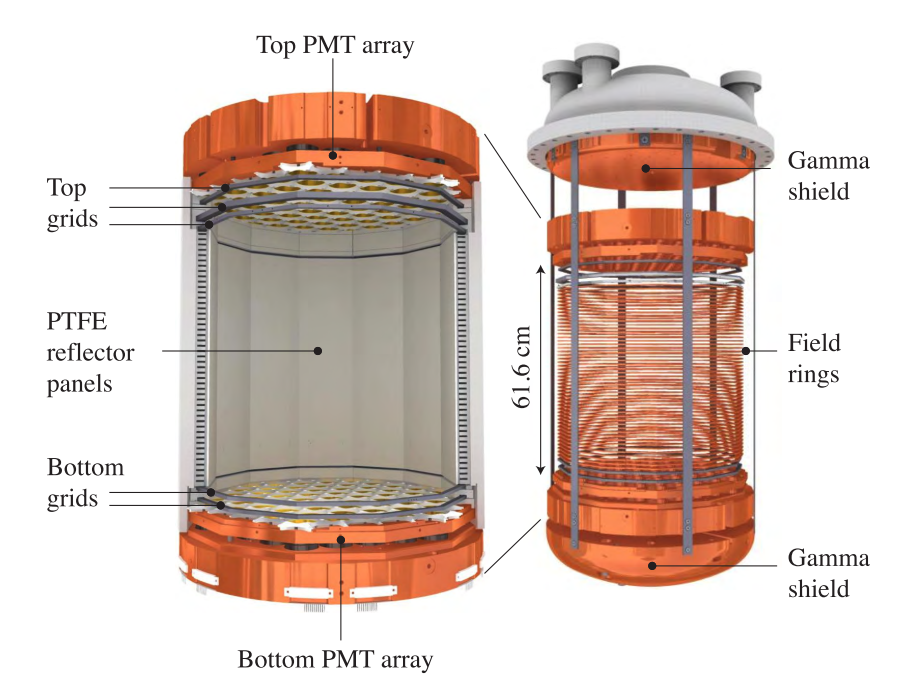
\includegraphics[width=\textwidth]{figures/lux/lux_inner2.png}
\caption{Field-shaping rings detail. Figure from \cite{LUXDetectorPaper}. }
\label{fig:lux2}
\end{center}
\end{figure}


More details about the internal components, including extensive characterization of the \ac{PMT}s, can be found in C. Faham's PhD thesis \cite{Faham2014a}.

\section{External Components}

The \ac{LUX} cryogenic system was based on thermosyphons, which deliver ``cooling power'' to solid copper cold heads, which are in thermal contact with the liquid xenon space. A simplified diagram is shown in Figure~\ref{fig:luxcryo}. A thermosyphon is a closed-loop cooling device containing a thermal messenger gas; N$_{2}$ was used in the \ac{LUX} thermosyphons. The top of the thermosyphon is immersed in a bath of liquid nitrogen, and the bottom is in thermal contact with the liquid xenon space. The internal messenger gas condenses at the top and drips down to the cold head, where it absorbs heat from the xenon space, evaporates, and returns to the top of the thermosyphon to condense and repeat the cycle. In this manner, heat from the liquid xenon space is transferred to the external nitrogen bath, which boils off and must be periodically replenished. The pressure of the internal nitrogen messenger gas can be adjusted, providing more or less cooling power as desired. The \ac{LUX} thermosyphons were also instrumented with resistive heaters, for further fine control. Four thermosyphons were used to operate the \ac{LUX} detector stably at \~175~K with a xenon vapor pressure of \~2~bar. 

\begin{figure}[htbp]
\begin{center}
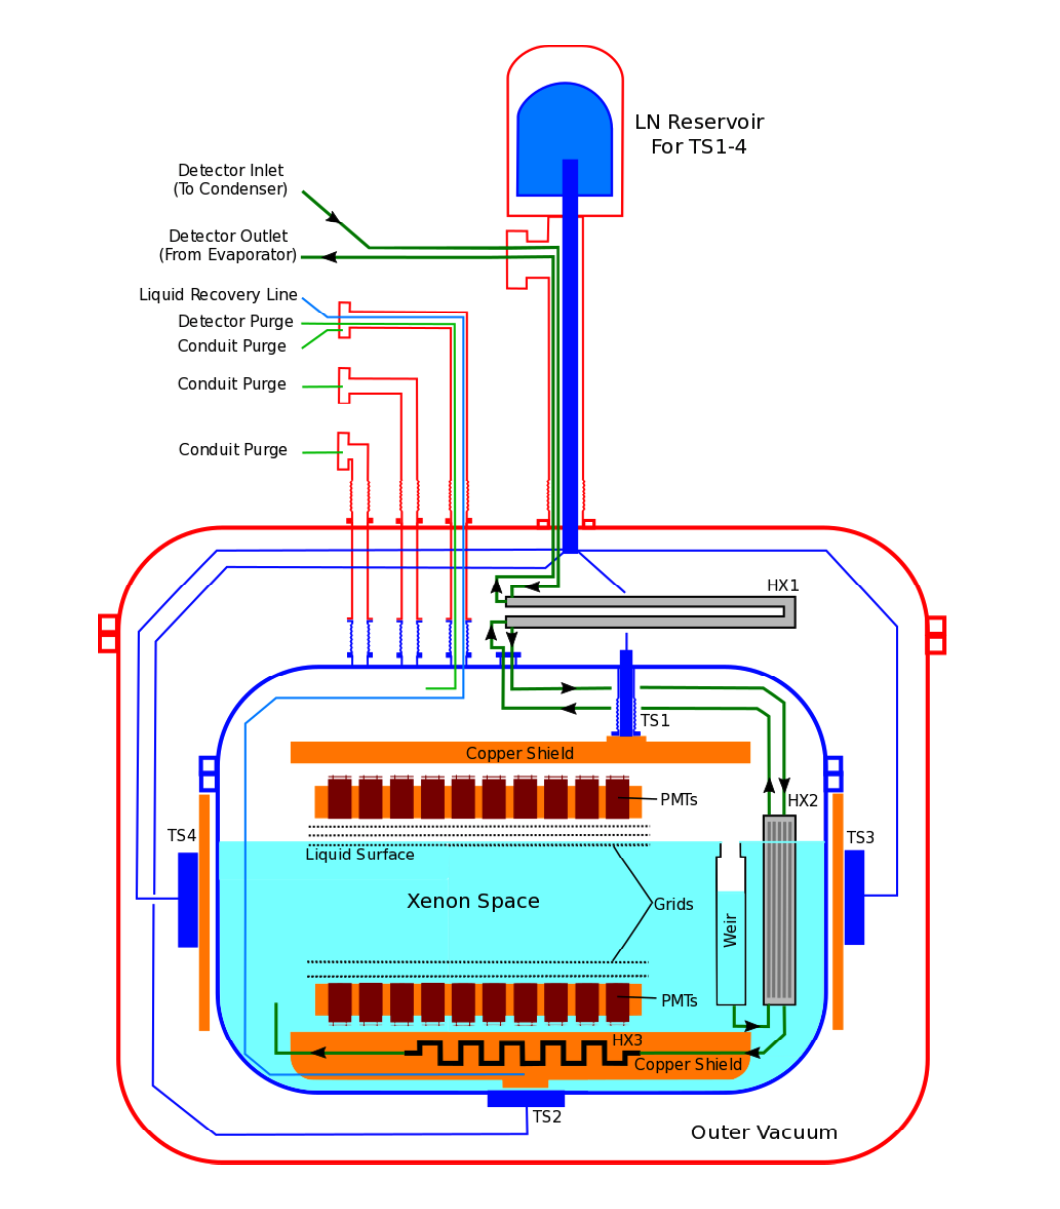
\includegraphics[width=\textwidth]{figures/lux/lux_cryostats.png}
\caption{A simplified diagram of the \acs{LUX} cryogenic system. Figure from \cite{Larsen2016}.}
\label{fig:luxcryo}
\end{center}
\end{figure}

The spillover liquid xenon from the liquid-level-setting weir mentioned above was directed into a circulation system through a series of heat exchangers that helped cool clean, incoming xenon gas. The xenon circulation was driven by one twin-head KNF double-diaphragm pump, which pushed liquid xenon from the spillover weir through a SAES MonoTorr heated zirconium getter to remove non-noble impurities before returning the clean xenon gas into the detector. A sampling system was able to pull xenon gas samples from different parts of the circulation system and measure impurity content, as well as test for the presence of $^{85}$Kr \cite{Dobi2011}, a troublesome beta emitter which must be removed from the xenon prior to carrying out a successful \ac{WIMP} search.

The circulation pump was installed in parallel with a backup pump, which could be switched on immediately in case of a pump outage. Flow was regulated to the system by two high-flow \ac{MFC}s. Additional low-flow \ac{MFC}s controlled purge flow through the cabling conduits in Figure~\ref{fig:luxcryo} to ensure gas flow was away from the detector and prevent any contaminants from diffusing into the active xenon space.

Internal calibration sources were plumbed into alternate flow paths of the circulation system. Xenon gas could be directed through a substrate source, such as the $^{83m}$Kr source described below, to pull $^{83m}$Kr into the detector volume. A bottle containing a source such as the CH$_{3}$T source described below could be used to deposit the gaseous source in an evacuated section of pipe. Xenon could then be directed through the section of pipe containing the source, sweeping it into the detector volume. 

Lastly, \ac{LUX} was placed in a 7.6~m diameter, 6.1~m high water tank (Figure~\ref{fig:luxwatertank}). The shielding provided by the water tank attenuated the $\gamma$ background from the cavern walls and thermalized neutrons from cavern background radioactivity and muon spallation. The water tank provided superior shielding from cavern radioactivity such that the detector backgrounds were dominated by the radioactivity of internal detector components, which in turn were controlled through a strict campaign of cleanliness and choice of detector materials \cite{LUXDetectorPaper}, \cite{LUXRun03Backgrounds}. Vertical tubes visible in Figure~\ref{fig:luxwatertank} were used to deploy external calibration sources at different heights, such as $^{137}$Cs, which were directed into the detector via a collimating source assembly.


\begin{figure}[htbp]
\begin{center}
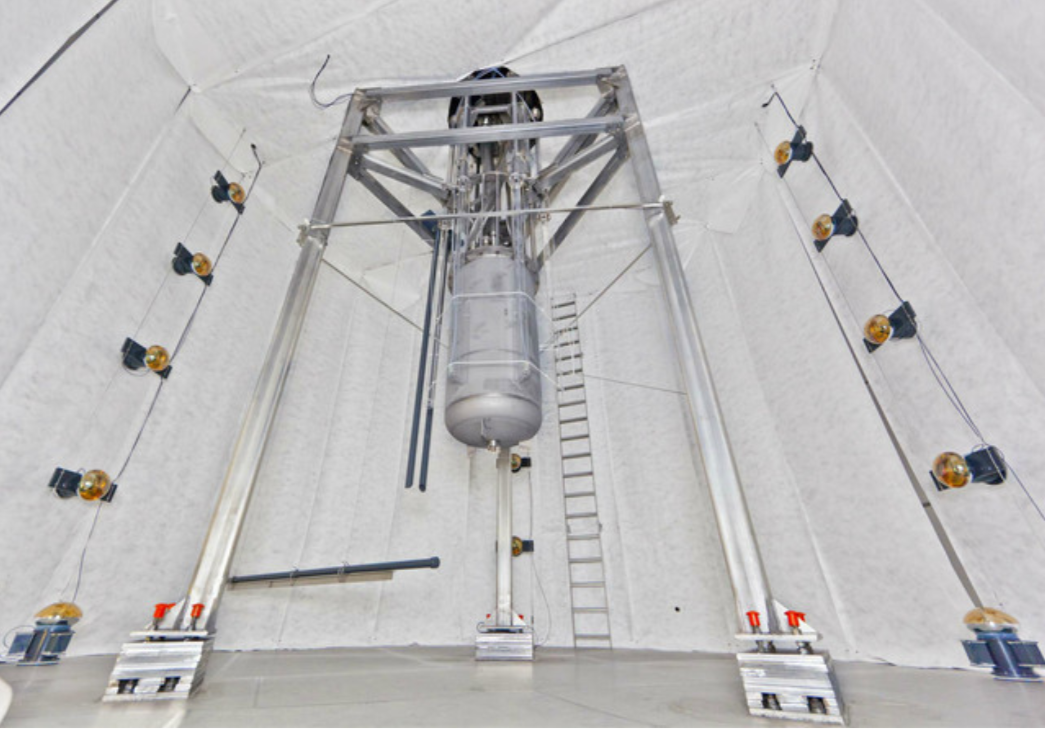
\includegraphics[width=\textwidth]{figures/lux/lux_watertank.png}
\caption{A photo of the \acs{LUX} detector installed inside the water tank. Photo credit Mark Kapust.}
\label{fig:luxwatertank}
\end{center}
\end{figure}

The \ac{LUX} detector water tank and material screening achieved a very low background in the \ac{WIMP} search energy range shown in Figure~\ref{fig:luxrun03bkg}. Figure~\ref{fig:luxrun03bkg} also illustrates the fiducial volume chosen for the Run03 \ac{WIMP} search.

\begin{figure}[htbp]
\begin{center}
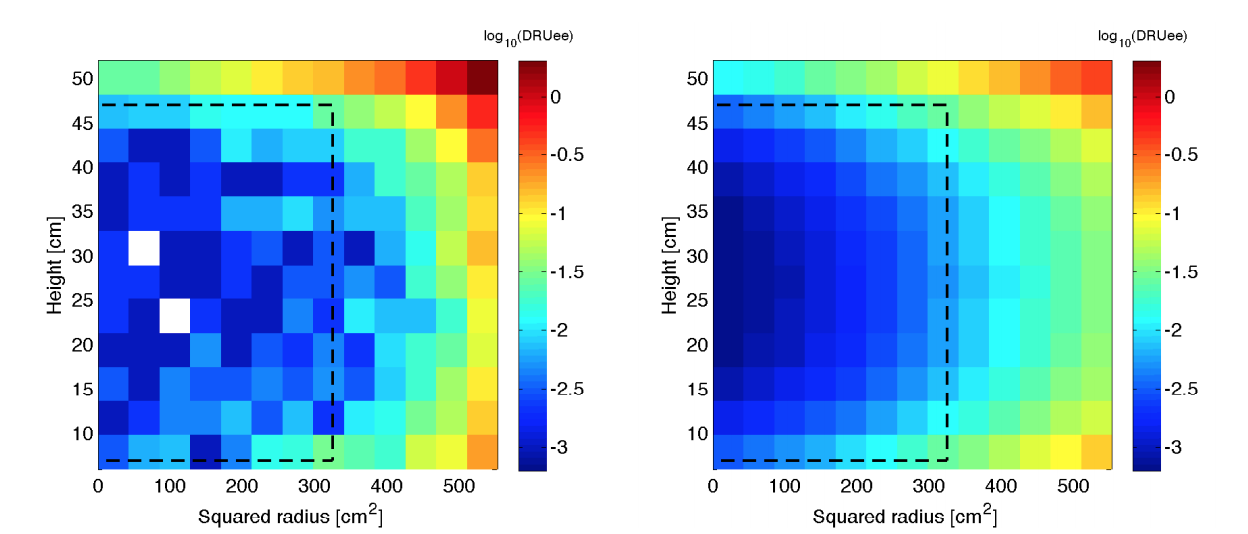
\includegraphics[width=\textwidth]{figures/lux/lux_run03bkg.png}
\caption{Backgrounds distributions in squared radius and height for expected (right) and measured (left) backgrounds in the energy range 0.9-5.3~keV$_{ee}$ (2-30 phe S1) for the 85.3 live-day Run03 \acs{WIMP} exposure. Black lines show the 118~kg fiducial mass. Units are log$_{10}$DRU$_{ee}$, electron equivalent differential rate units, i.e. keV$_{ee}^{-1}$kg$^{-1}$day$^{-1}$.  Figure from \cite{LUXRun03Backgrounds}. }
\label{fig:luxrun03bkg}
\end{center}
\end{figure}


\section{Trigger and Data Acquisition}
Cabling for \ac{PMT}s and other monitoring instrumentation were routed from the inner detector volume to the outside via conduits illustrated in in Figure~\ref{fig:luxcryo}. A flow chart illustrating the signal path is shown in Figure~\ref{fig:luxdaq}. 

\begin{figure}[htbp]
\begin{center}
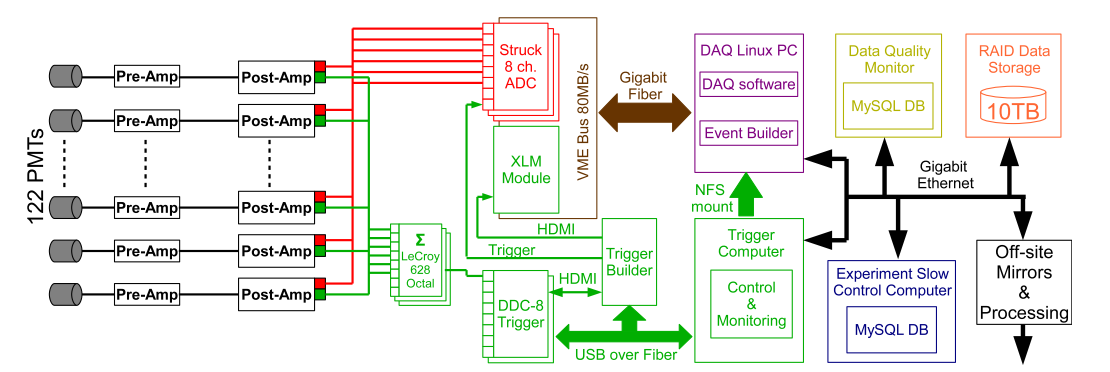
\includegraphics[width=\textwidth]{figures/lux/lux_daq.png}
\caption{Overview of the \acs{LUX} trigger system. Figure from \cite{LUXTrigger}. }
\label{fig:luxdaq}
\end{center}
\end{figure}


The \ac{PMT} signals were shaped and amplified by two sets of amplifiers. These analog voltage waveforms were then digitized by Struck \ac{ADC}s, with 14 bit, 100~MHz sampling (1 sample every 10~ns). A copy of the analog \ac{PMT} voltage waveforms passed through the \ac{LUX} \ac{FPGA} trigger system, which signaled the data acquisition computer to save the waveforms when they passed above a certain threshold, and stop when they fell below the threshold. Each of the 122 \ac{PMT}s was dedicated its own channel in the recorded data, so recording only the channels\footnote{The Struck boards actually acquired channels in pairs. Each channel had a dedicated parter, and if one of the channels exceed the \acs{POD} threshold, both partner channels were acquired.} that passed threshold allowed for a great amount of data reduction. This technique is called \ac{POD}. A \ac{POD} threshold of 1.5~mV was used for \ac{LUX}, which resulted in a single photoelectron efficiency of > 95\% \cite{LUX:Run03Comprehensive}. A figure showing the \ac{POD} threshold and example waveform are shown in Figure~\ref{fig:waveforms}. More details about the \ac{LUX} data acquisition system can be found in \cite{LUXDAQ}. 


\begin{figure}[htbp]
\begin{center}
%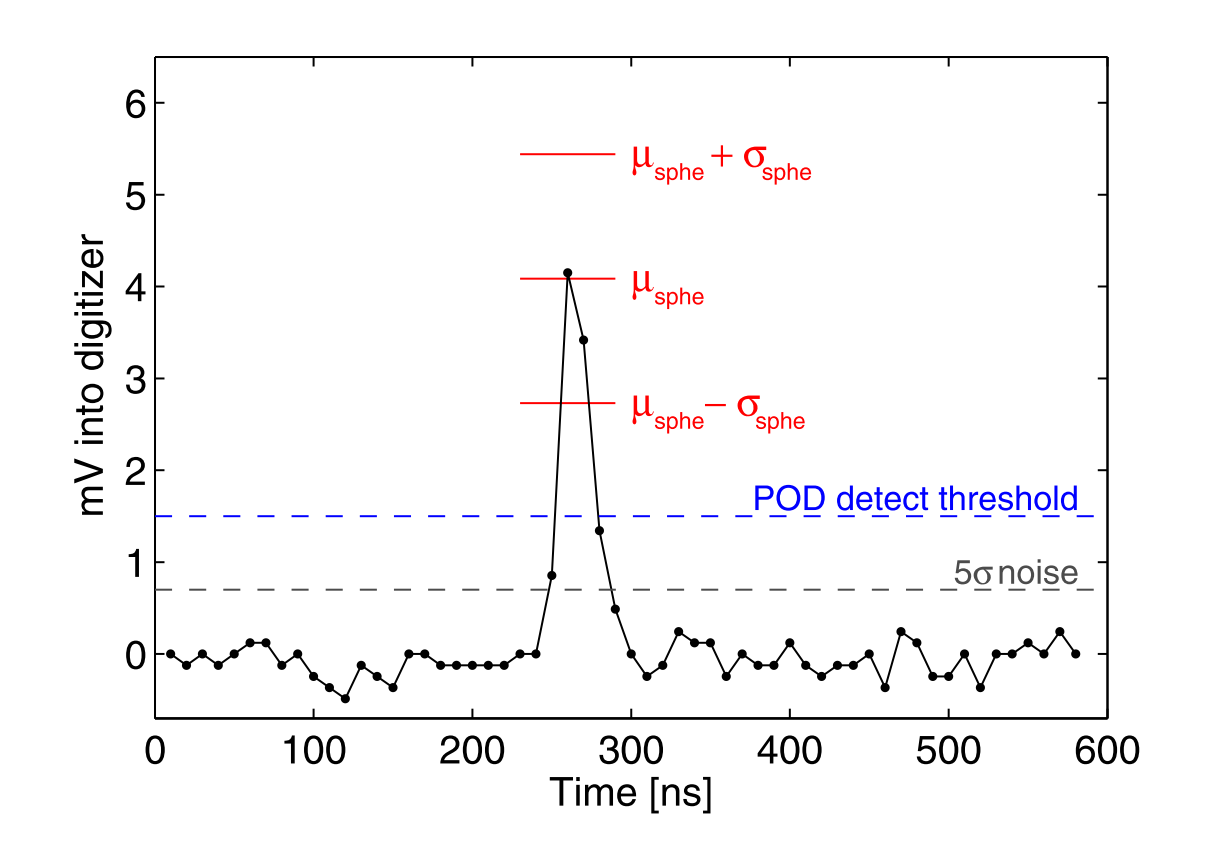
\includegraphics[width=0.29\textwidth]{figures/lux/pod_detect.png}
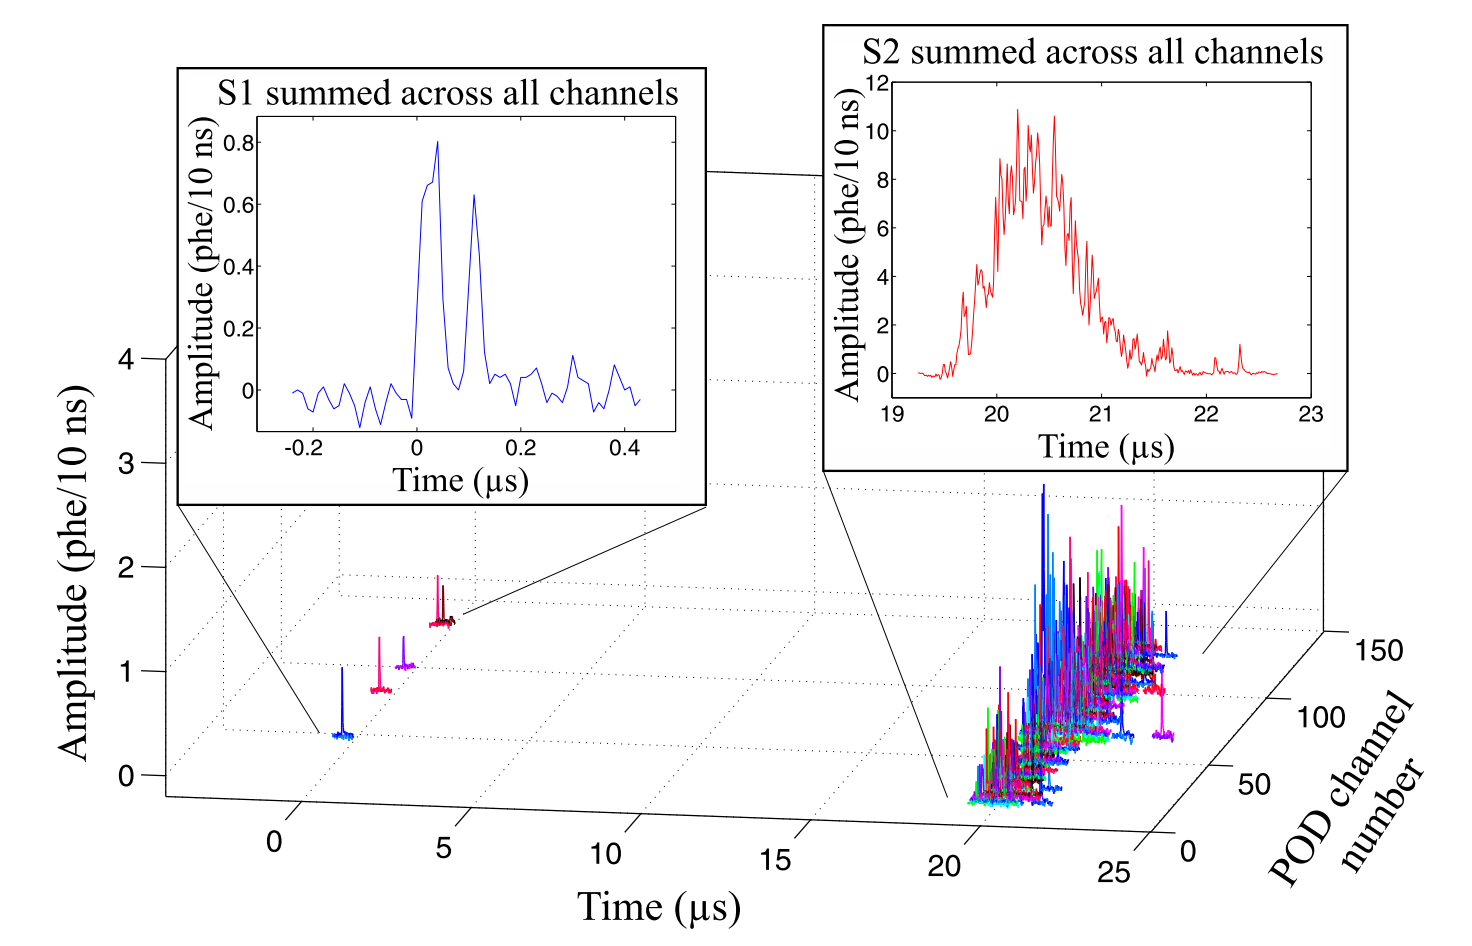
\includegraphics[width=\textwidth]{figures/lux/sample_waveform.png}
\caption{An example recorded event. Channels that do not pass the POD threshold are not recorded. The waveforms are summed over all channels to produce the S1 and S2. Figure from \cite{LUXTrigger}. }
\label{fig:waveforms}
\end{center}
\end{figure}

The channel-wise \ac{POD} data was written continuously to disk as the \ac{ADC} memory buffer fills; this is the rawest and least filtered form of \ac{LUX} data that is saved in binary format (referred to as ``\textbf{.dat}-files''). Upon receiving a trigger signal, the Event Builder takes the takes the raw data and extracts portions located in a pre-trigger and post-trigger window. A additional hold-off time is applied after the post-trigger window to assure \ac{POD}s are not duplicated the subsequent event. More details about the trigger can be found in \cite{LUXTrigger}. The pre- and post- trigger windows for Run03 were set to be 500~$\mu$s, chosen to ensure both S1 and S2 pulses were contained in the same event. The maximum electron drift time in Run03 was 322~$\mu$s, so a pre- and post- trigger time of 500~$\mu$s ensured no S2 would appear without its partner S1. Both S1 and S2 could pass the \ac{POD} threshold and signal the \ac{DAQ} computer to save the waveforms, but some small S1s may not have crossed the trigger threshold and were ``found'' only at the event-building stage. After event-building, the waveform data was again saved in binary format. These files containing waveforms that are associated with individual events, are referred to as ``\textbf{.evt}-files''.


\section{Data Processing}
\label{sec:lux_dpf}
After event-building, the waveform \textbf{.evt}-files were sent off site for additional processing. The \ac{LUX} \ac{DPF} extracts essential information from the waveforms and produces \ac{RQ} files (referred to as ``\ac{RQ} files''). The \ac{DPF} is modular, and can be applied repeatedly to the same \textbf{.evt}-files with different settings if desired. \ac{RQ} files include event-level information (e.g. trigger timestamp), pulse-level quantities (e.g. pulse type, pulse area), and some channel-level quantities (e.g. pulse area recorded by each \ac{PMT}). The \ac{DPF} classifies pulses as one of five types: S1, S2, \ac{SPHE}, \ac{SE}, and Else (for pulses that do not fit one of the previous four types). The pulse-finding and classification algorithm was designed and optimized for the \ac{WIMP} search, and is crucial in identifying \ac{WIMP} ``golden events'', which are single-scatter interactions with only one S1 and one S2 in the event. Detector backgrounds such as gammas often scatter more than once in the active volume, producing an event with one S1 and multiple S2s. The pulse-finder and classifier also play a large role in \ac{LIP} search, which is discussed more in Chapter~\ref{ch:lips}. An example of pulse identification for a multiscatter event is shown in Figure~\ref{fig:lux_pulses}.

\begin{figure}[htbp]
\begin{center}
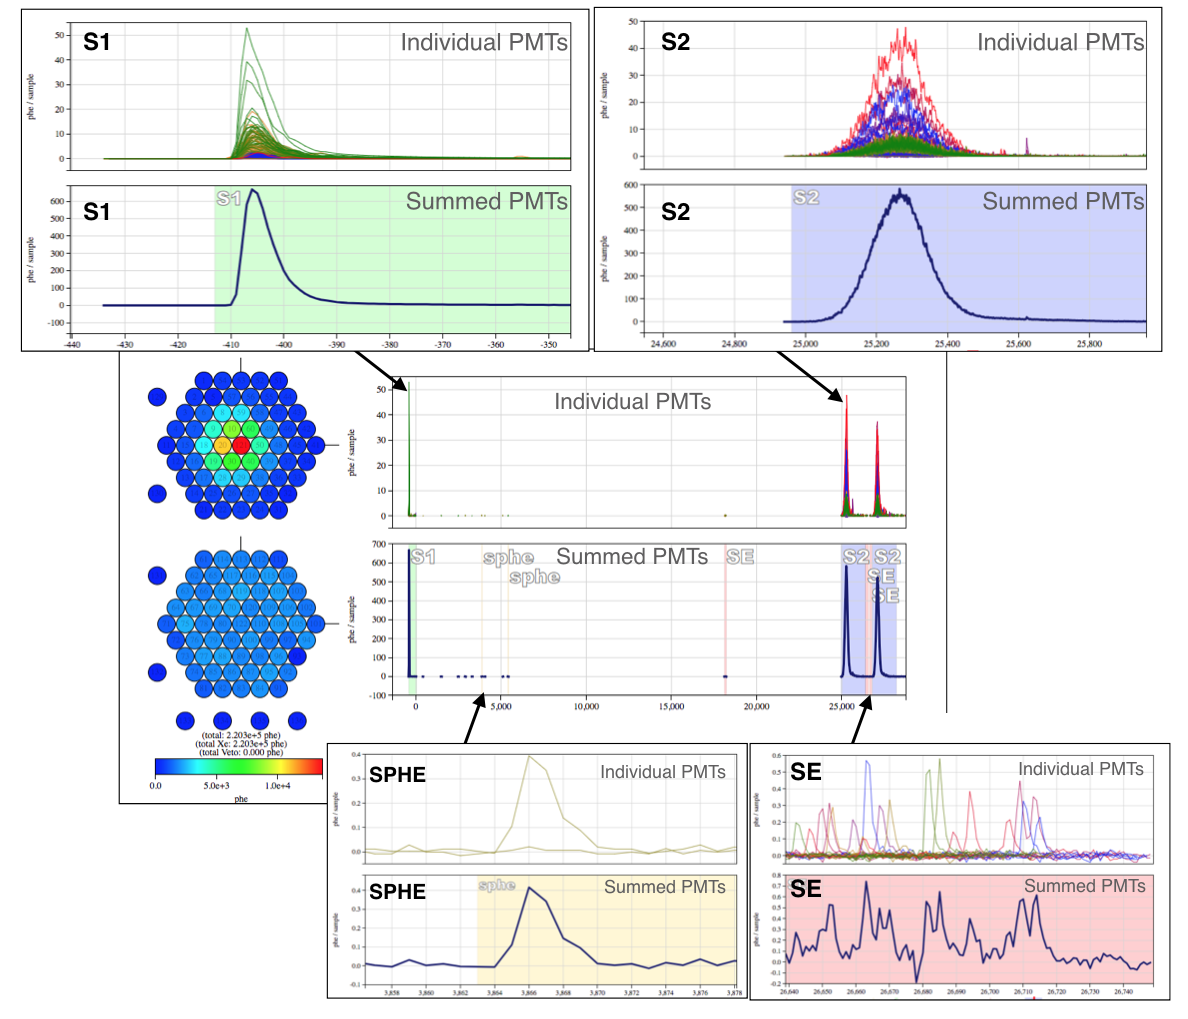
\includegraphics[width=\textwidth]{figures/lux/lux_pulses.png}
\caption{An example of \acs{LUX} pulse classification from a multiscatter event showing detail of individual pulses of types S1, S2, SPHE, and SE. In addition to the pulse classes illustrated here, there is an Else class, for pulses that do not fit any of the definitions shown. }
\label{fig:lux_pulses}
\end{center}
\end{figure}


Following identification of S1 and S2 pulses, the \ac{DPF} position reconstruction module is run. This module uses the Mercury algorithm, originally developed for the ZEPLIN-III \ac{LXe} \ac{TPC} \cite{Currie2012}, which is based on maximum-likelihood to find the best ($x,y$) position of the event. Mercury uses \ac{LRF}s, obtained for each \ac{PMT}, to predict the response of the \ac{PMT} to interactions at some arbitrary distance from the \ac{PMT}. The \ac{LRF}s were obtained using calibration data, of which $^{83m}$Kr was the most important for position reconstruction. The position reconstruction method and \ac{LRF}s are discussed in more detail in \cite{LUXPositionReconstruction}.


The \ac{DPF} also applies calibration constants to the data. Calibration constants, many of which change over time, are tracked and recorded in the \ac{LUG}, which produces date-specific record files in XML format, which in turn determine the settings for some of the \ac{DPF} modules. For example, the $^{83m}$Kr calibration (see Section~\ref{sec:krypton}) was used to normalize S1 pulse areas. The photon detection efficiency for S1s varies with $z$-position. Events occurring near the bottom \ac{PMT}s were \~50\% more likely to be detected than those near the liquid-gas boundary. The \ac{DPF} applies corrections like this to several \ac{RQ}s, and both the corrected and uncorrected versions are kept in the \ac{RQ} files. 


\section{Calibrations}
Several novel calibration methods were developed by the \ac{LUX} Collaboration to fully characterize the detector. The superior self-shielding ability of \ac{LXe} detectors also makes them difficult to calibrate. Sources placed external to the detector cannot penetrate the fiducial volume very effectively; since high-statistics are desired for calibration data, relying on external sources becomes untenable. The solution, then, is counterintuitive: purposely introduce radioactive material into the painstakingly developed, ultra low-background, fiducial volume of the detector. For such a source to not destroy the ability to carry out a \ac{WIMP} search, it must either (i) be short lived or (ii) be effectively removed by getter on a short timescale. \ac{LUX} demonstrated that $^{83m}$Kr fit the former \cite{LUXKr} requirement and tritiated methane (CH$_{3}$T) fit the latter \cite{LUXTritium}. Both of these sources were used in the calibration of the \ac{LUX} detector, in addition to other sources; all of the sources are discussed below. 

\subsection{Energy Reconstruction}
This section covers the energy calibration of \ac{LUX}. Recall from Chapter~\ref{sec:energy_reconstruction} that the electron-equivalent energy of an event in a dual phase xenon \ac{TPC} is reconstructed as follows:

\begin{equation}
E = W \Big(\frac{S1}{g_{1}} + \frac{S2}{g_{2}}\Big)
\end{equation}

Two or more calibration line sources of different energies are required to fit for the detector gains $g_{1}$ and $g_{2}$. The \ac{LUX} experiment used a suite of sources to calibrate the energy response of the detector, shown in Figure~\ref{fig:calib_sources}. The $^{83m}$Kr is an injected source distributed in the entire internal volume (discussed in more detail below). The $^{137}$Cs is an external source lowered at different heights into the source tubes. The xenon lines, $^{131}$Xe, $^{129}$Xe $^{127}$Xe, are internal sources of cosmogenic origin and were only present early in Run03.

\begin{figure}[htbp]
\begin{center}
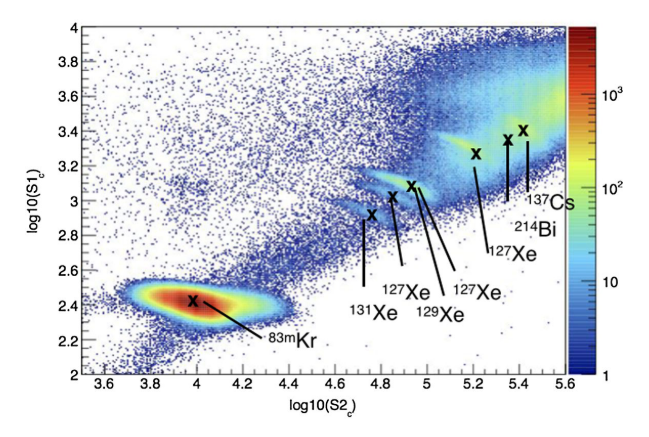
\includegraphics[width=\textwidth]{figures/lux/calibration_sources.png}
\caption{Plot showing calibration sources used for determination of the detector gains, $g_{1}$ and $g_{2}$. The axis label subscript $c$ denotes corrected variables with calibration for geometrical effects and electron lifetime; these corrections are discussed in Section~\ref{sec:krypton}. Figure from \cite{LUX:Run03Comprehensive}.}
\label{fig:calib_sources}
\end{center}
\end{figure}

The average S1 and S2 of each calibration source is normalized to the true energy:

\begin{equation}
(S1, S2) \longrightarrow \Big(\frac{\langle S1 \rangle}{E}, \frac{\langle S2 \rangle}{E}\Big)
\end{equation}

and a line $y = mx + b$ is fit to the transformed variables, where the slope is $m = -g_{1} / g_{2}$ and the y-intercept is $b = g_{1} / W$. Such a plot is called a Doke plot. The sources from figure Figure~\ref{fig:calib_sources} are shown normalized in a Doke plot in Figure~\ref{fig:doke}.

\begin{figure}[htbp]
\begin{center}
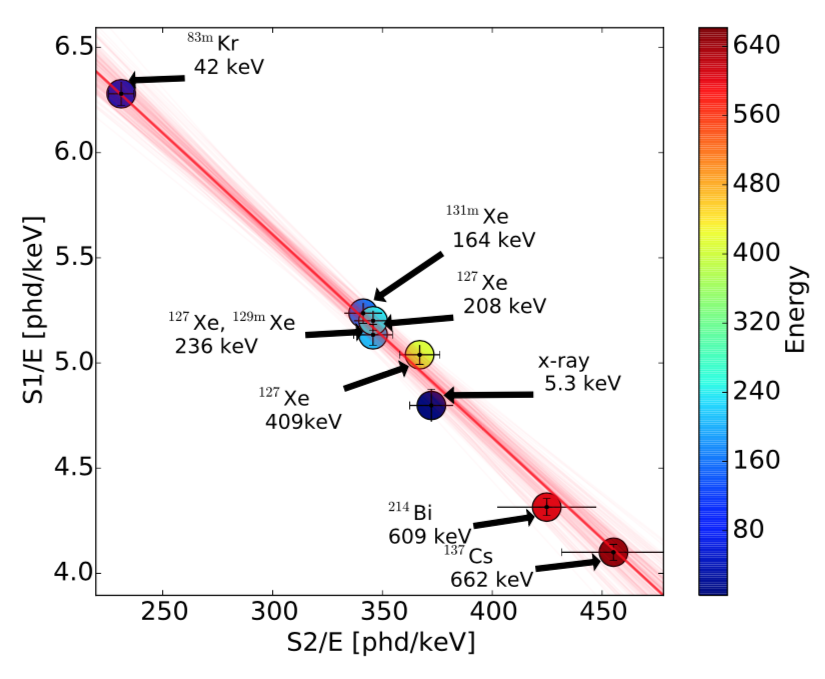
\includegraphics[width=\textwidth]{figures/lux/doke.png}
\caption{ Doke plot used to fit for $g_{1}$ and $g_{2}$ in \acs{LUX} Run03. Figure from \cite{LUX:Run03Comprehensive}.}
\label{fig:doke}
\end{center}
\end{figure}

From the fit in Figure~\ref{fig:doke}, the \ac{LUX} gains for Run03 were measured to be $g_{1} = 0.117 \pm 0.003$~phd/photon and $g_{2} = 12.1 \pm 0.8$~phd/electron. $g_{2}$ depends on a combination of the \ac{EEE} and the number of photons produced by a single extracted electron -- it is useful to know both values. Single electrons are periodically emitted into the gas and undergo proportional scintillation. This phenomenon is well known in liquid xenon detectors and is discussed further in Chapter~\ref{ch:etrains}. A sample of pure single electrons was collected to find the average number of S2 photons produced by one electron, referred to the single electron size. The single electron size in Run03 was a skew-gaussian with mean 24.66~phd and a 1-$\sigma$ width of 5.95~phd. Combing this with $g_{2}$ gives an \ac{EEE} of $49\% \pm 3\%$ \cite{LUX:Run03Comprehensive}.

\subsection{Metastable Krypton-83 ($^{83m}$Kr): A Multifunction Calibration}
\label{sec:krypton}
The $^{83m}$Kr source used by \ac{LUX} was $^{83}$Rb deposited on a charcoal substrate. Gaseous xenon within the circulation system was diverted over the charcoal substrate, where it could sweep $^{83m}$Kr on a flow path through the getter, and then into the detector. 

$^{83m}$Kr decays by two steps releasing a total energy of 41.5~keV (see Figure~\ref{fig:kr_decay} ). The two branching ratios that dominate are, first, the internal conversion and subsequent Auger emission of a 32.1~keV $\beta$ followed by another internal conversion and Auger emission of a 9.4~keV $\beta$, with an intervening half-life of 154~ns. The time structure of the decay sometimes yielded two S1s, called S1a and S1b. If the second 9.4~keV $\beta$ was prompt (i.e within the timing resolution of the detector), then only one S1 was observed. The S2s were always merged because (1) the low energy of the decays made the energy depositions O(10~$\mu$m) from each other, smaller than the position resolution of the detector O(1~mm) and (2) the close timing of the two decays was smaller than the typical electron diffusion distances during drift O(1~mm), merging the two electron bunches together into one S2 \cite{LUXKr}.

\begin{figure}[htbp]
\begin{center}
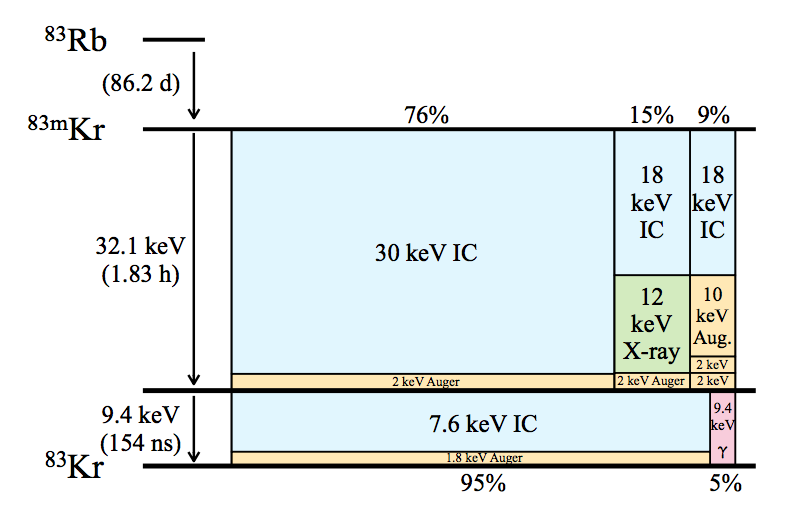
\includegraphics[width=\textwidth]{figures/lux/kr_decay.png}
\caption{ Decay scheme of $^{83m}$Kr. The width of each column is proportional to the branching fraction of that decay mode, the vertical divisions are proportional to energy partitioning among internal conversion electrons (blue), Auger electrons (yellow), x rays (green), and gamma rays (red). In the \acs{LUX} detector, the S1s of the 32.1~keV $\beta$ and the 9.4~keV $\beta$ were sometimes separable, the S2s were always merged. If the S1s were separate they were referred to as S1a and S1b. Figure from \cite{LUXKr}.}
\label{fig:kr_decay}
\end{center}
\end{figure}


$^{83m}$Kr was a workhorse calibration source for \ac{LUX}, with $^{83m}$Kr injections performed weekly at activities ranging from ~10~Bq to hundreds of Bq, depending on the specific calibration goal. $^{83m}$Kr was found to mix uniformly in the detector within \~10~min of the injection, and would decay (half life 1.83~hours) back to an acceptable \ac{WIMP} search background rate within a day, or few days, depending on the injected activity \cite{LUXKr}. The combined energy of the $^{83m}$Kr was well out of the \ac{WIMP} search energy range, so no long-term pollution, though unlikely, was risked. $^{83m}$Kr was used for two main calibrations, described below.

\textbf{Pulse Area Corrections} Detector efficiencies and gains can vary over time and position within the detector. $^{83m}$Kr served as a ``standard candle'', which produced monoenergetic signals with uniform initial light and charge yields distributed uniformly throughout the active volume. The efficiency for detecting the initial light yield as an S1 was dominated by spatially varying geometrical light detection efficiency. The areas of the S1s were binned in 3D, and the averages were found for each bin. A correction map was then constructed as the inverse of the S1 areas, normalized to the S1 amplitude at the center of the detector. The map of relative S1 amplitudes in Figure~\ref{fig:kr_1} (left) shows the strong $z$-dependance for S1 light collection. The corrections for S2 areas were more complex, as detection efficiency for the initial charge yield of an S2 depends on the presence of electronegative impurities, electron extraction efficiency, production of proportional scintillation photons, and detection of those photons in \ac{PMT}s. The $xy$- and $z$- dependence for S2s are corrected in two separate maps. The electronegative impurities caused a strong z-dependence in S2 size -- events originating at the bottom of the detector must drift longer and so were more likely to encounter and lose electrons to impurities. The $z$-dependent S2 area correction map was an exponential function of drift time, normalized to unity at the liquid surface. The $xy$-dependence was from detector conditions such as pressure, liquid level, and electric field variation from the grid. The $xy$-correction map for S2s was normalized to (0,0) in the x-y plane. Examples of both the $z$ and $xy$ S2 area correction maps can be seen in Figure~\ref{fig:kr_1} (right).

\begin{figure}[htbp]
\begin{center}
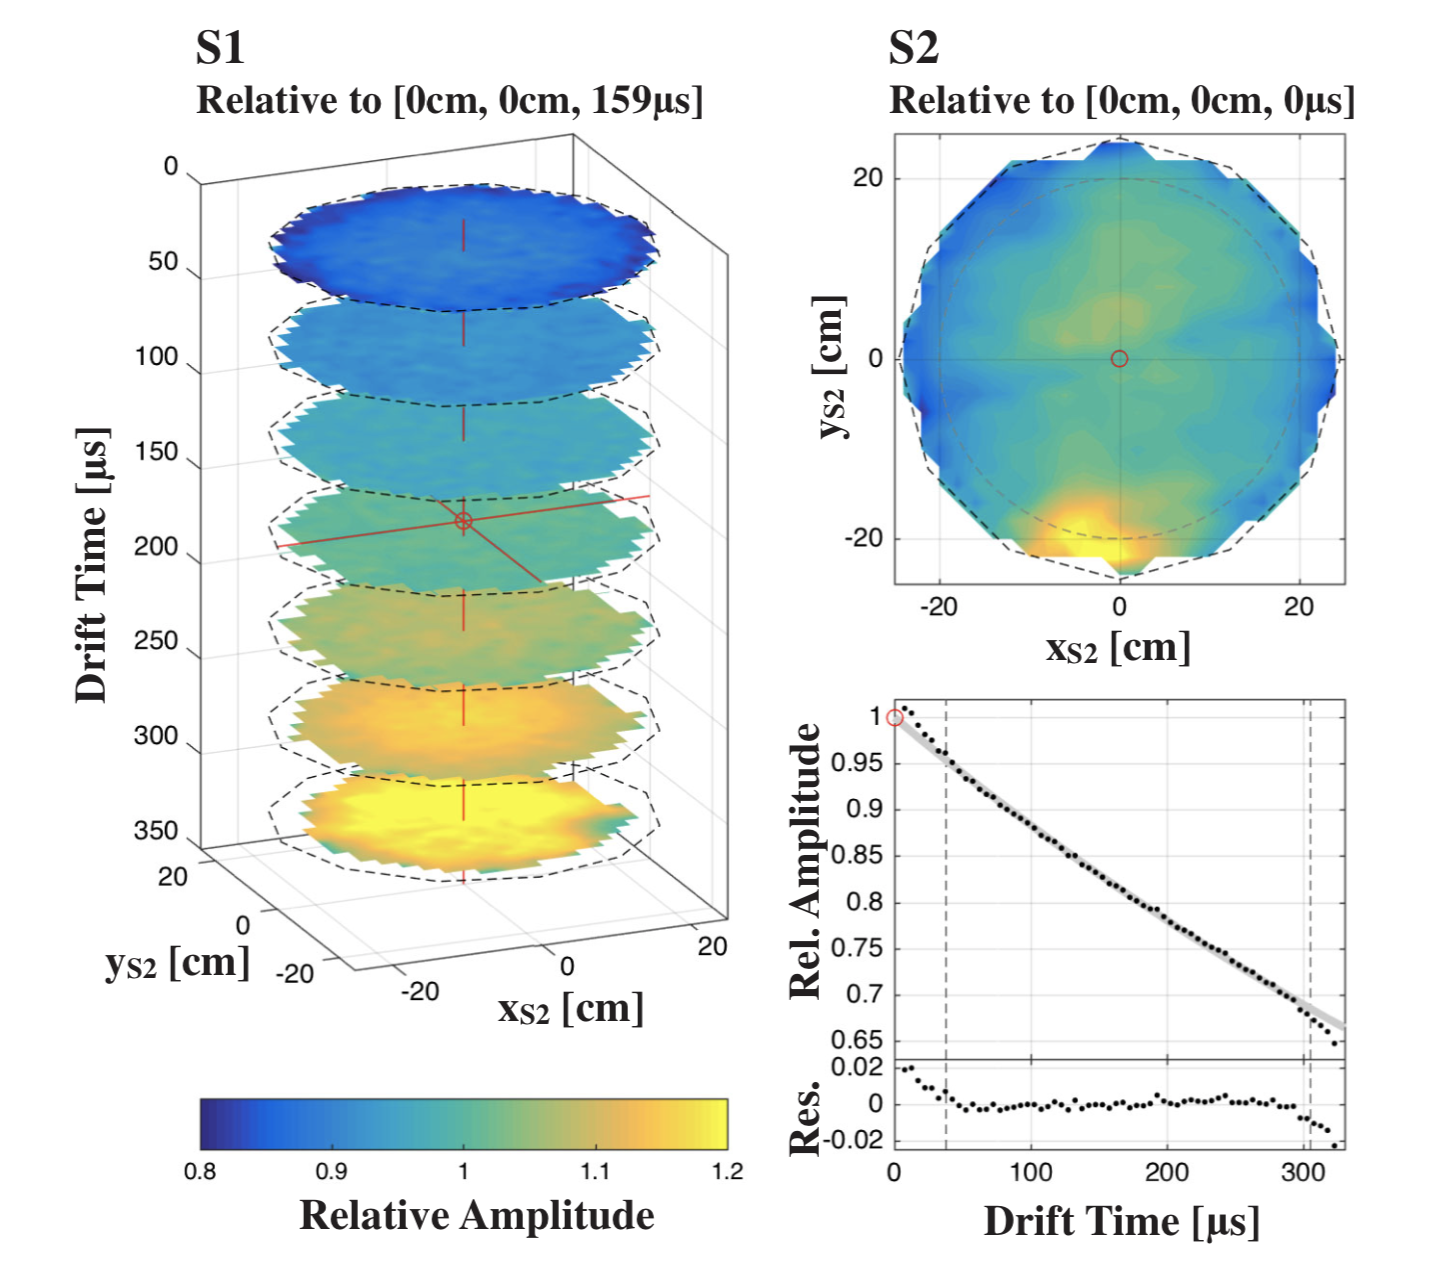
\includegraphics[width=\textwidth]{figures/lux/kr_1.png}
\caption{ Spatial dependence of pulse area corrections for S1 (left) and S2 (right) from an example $^{83m}$Kr calibration. The red circle indicates normalization point. Figure from \cite{LUXKr}}
\label{fig:kr_1}
\end{center}
\end{figure}

\textbf{Position Corrections} 3D position reconstruction depends on a full understanding of the path electrons take from an interaction site to the position observed after extraction at the surface. The reconstructed position of the proportional scintillation signal in the $xy$-plane, based on the Mercury algorithm, is referred to ``S2 coordinates", often with subscripts (x$_{S2}$, y$_{S2}$). The real coordinates may be displaced from (x$_{S2}$, y$_{S2}$) due to, for example, a radial field pushing electrons inwards deep in the detector. In fact, there was a small radially inward component to the electric fields in \ac{LUX} Run03 due to the geometry of the field cage and grids (Figure~\ref{fig:kr_pos1}). The spatial distribution of reconstructed $^{83m}$Kr events was used to verify a COMSOL multiphysics electric field model of the detector by drifting electrons in simulation under the electric field model conditions. This field model could then be used to transform events from S2 coordinates to real ($x,y$) coordinates, however this was not done for Run03. Instead, the $^{83m}$Kr data itself was found to be more precise for position corrections, since it didn't rely on the accuracy of the field model or electron drift simulation (Figure~\ref{fig:kr_pos2}). The electric field conditions were very different in Run04, and so extensive calibrations and field maps were used to map S2 coordinates to real coordinates \cite{LUXFields}.

\begin{figure}[htbp]
\begin{center}
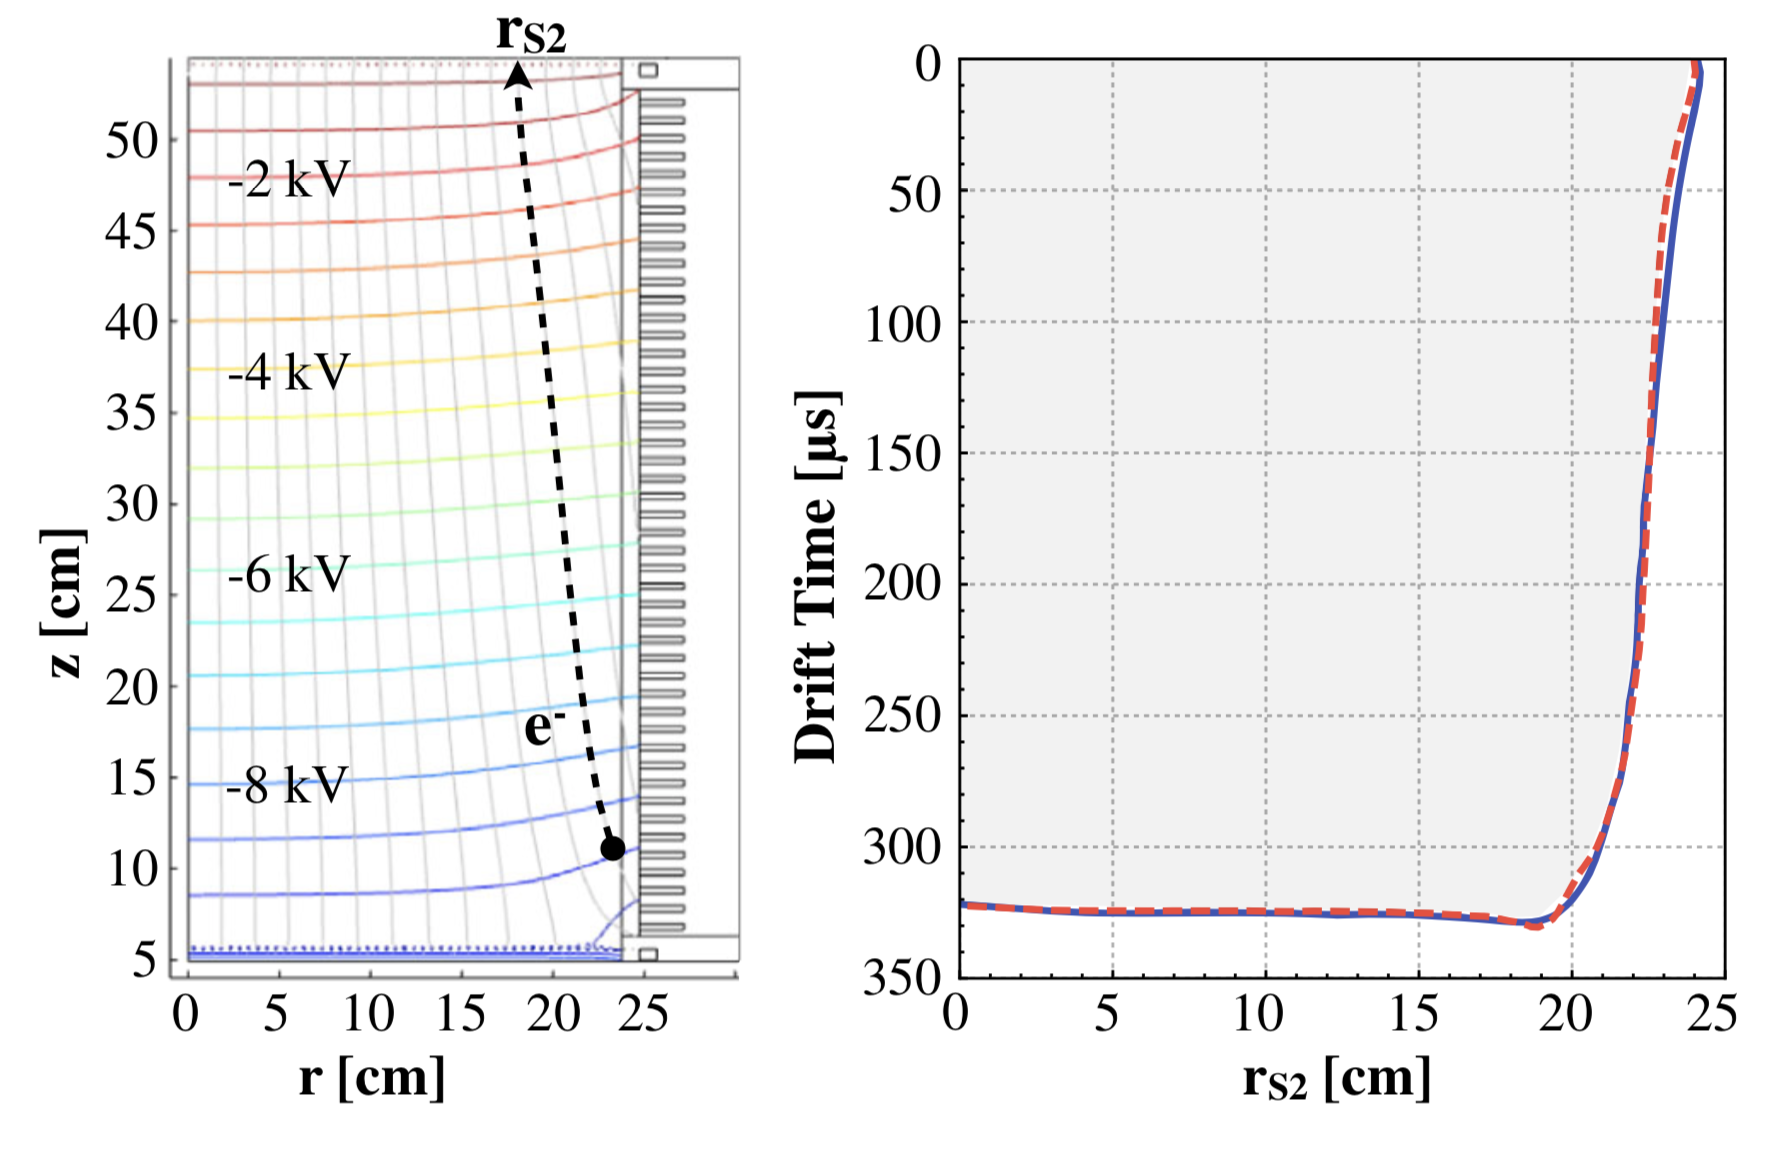
\includegraphics[width=.8\textwidth]{figures/lux/kr_pos1.png}
%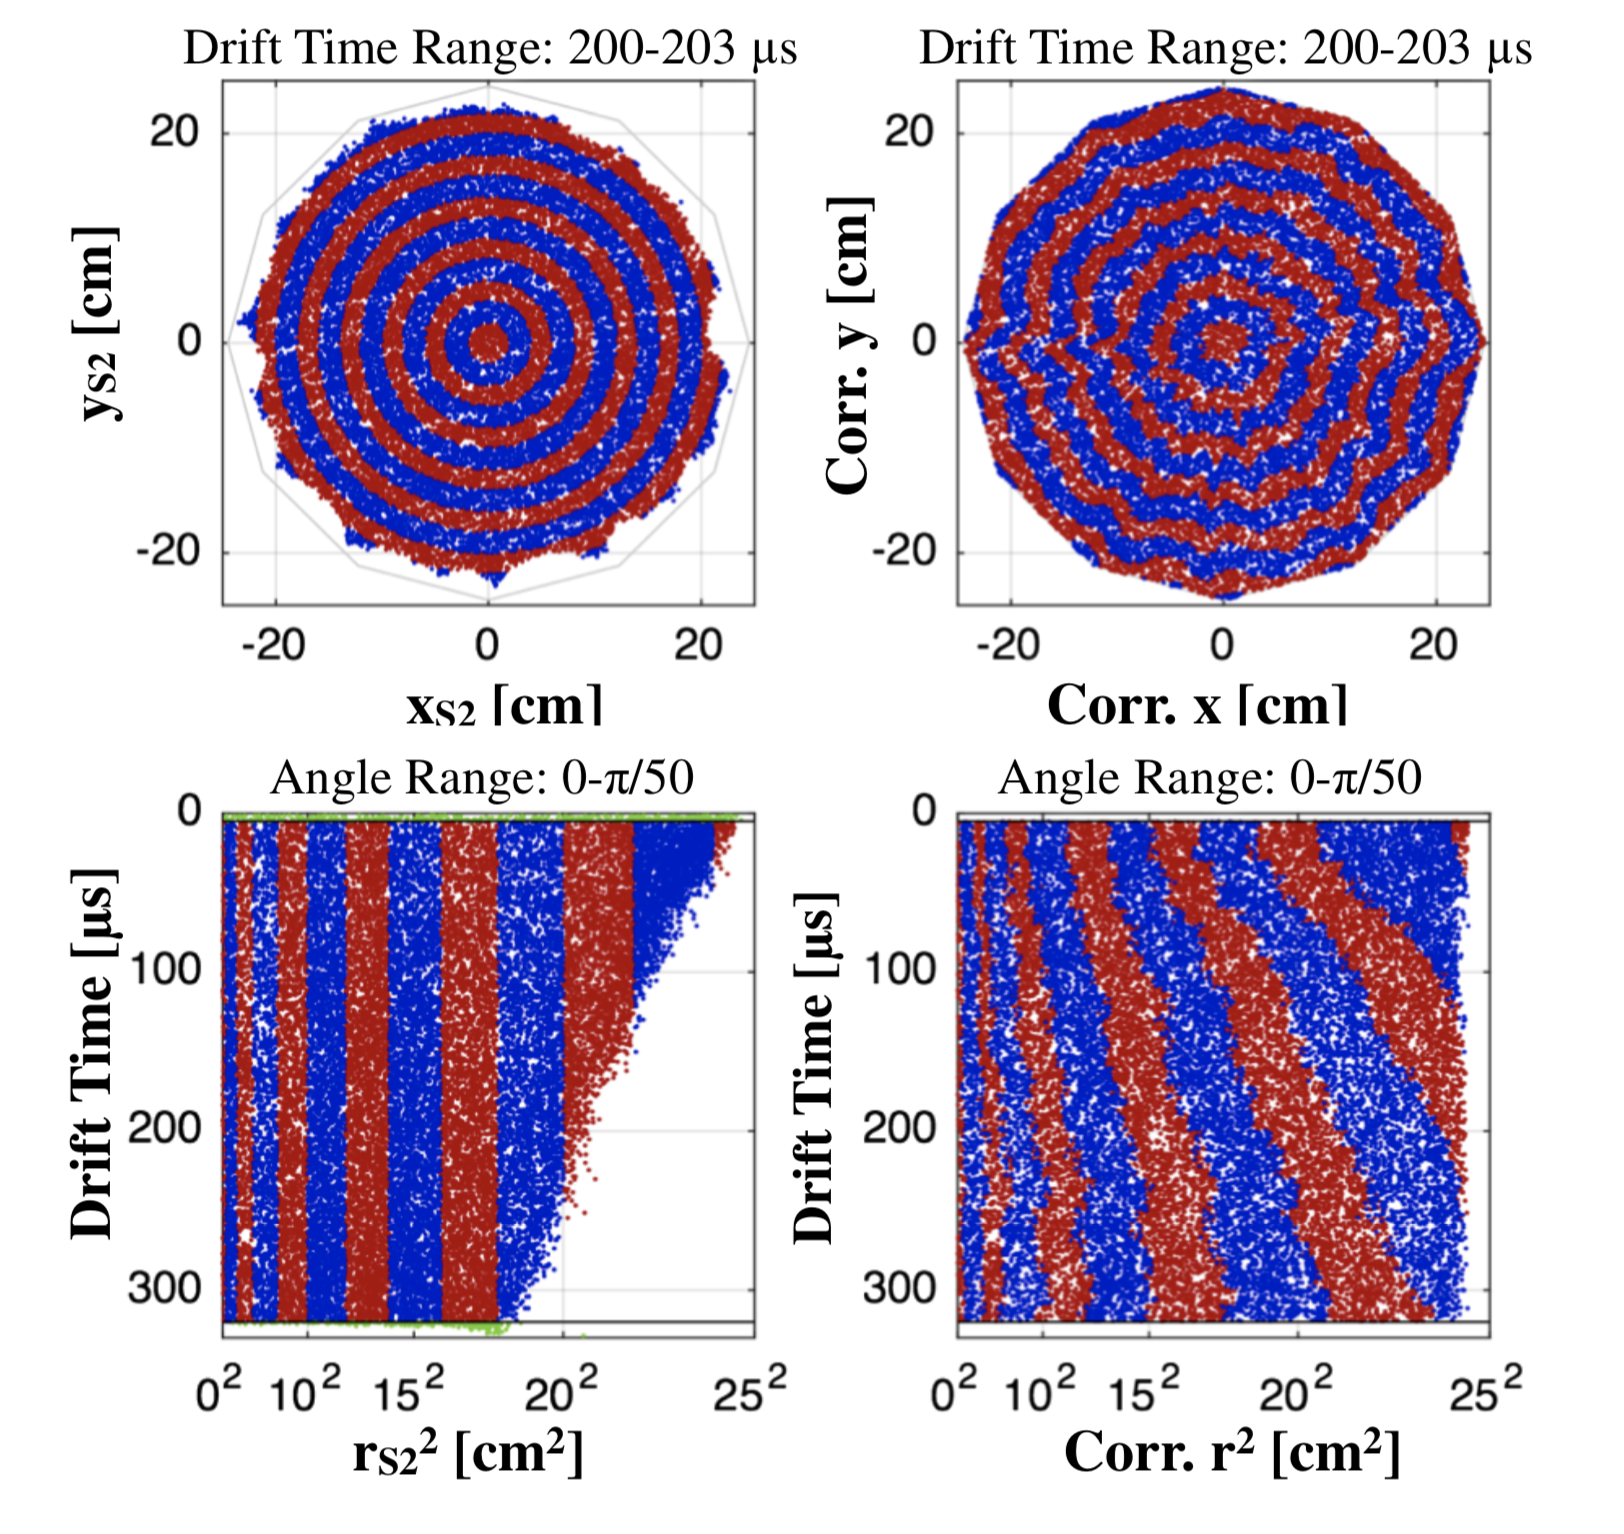
\includegraphics[width=\halffig]{figures/lux/kr_pos2.png}
\caption{ (left) A simplified 2D COMSOL model showing electric field lines and equipotentials for the \acs{LUX} detector in Run03. A radially inward component is seen. (right) The resulting edge S2 coordinates of a uniform distribution of electrons drifted under the electric field model is shown in solid blue. The edge S2 coordinates of from $^{83m}$Kr data is in dashed red; it is consistent with the field model prediction. Figure from \cite{LUXKr}.}
\label{fig:kr_pos1}
\end{center}
\end{figure}

\begin{figure}[htbp]
\begin{center}
%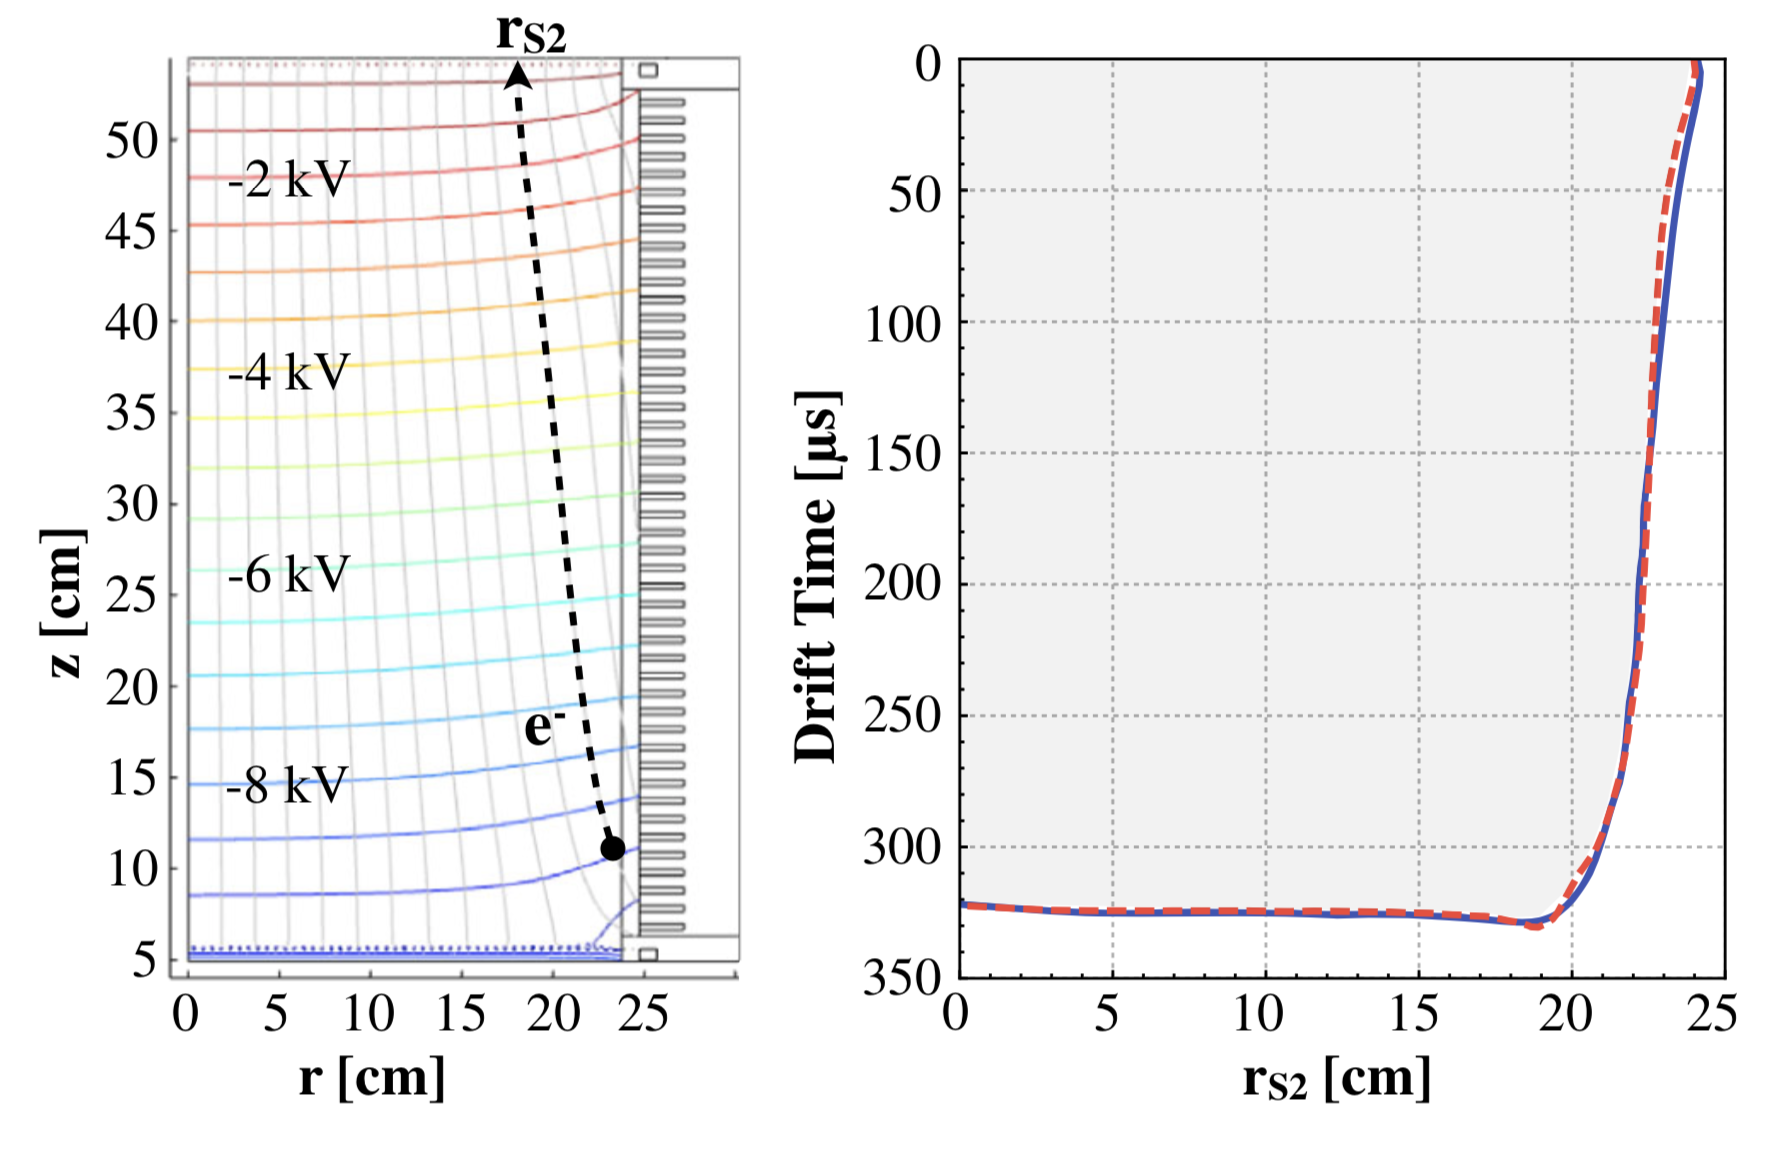
\includegraphics[width=\halffig]{figures/lux/kr_pos1.png}
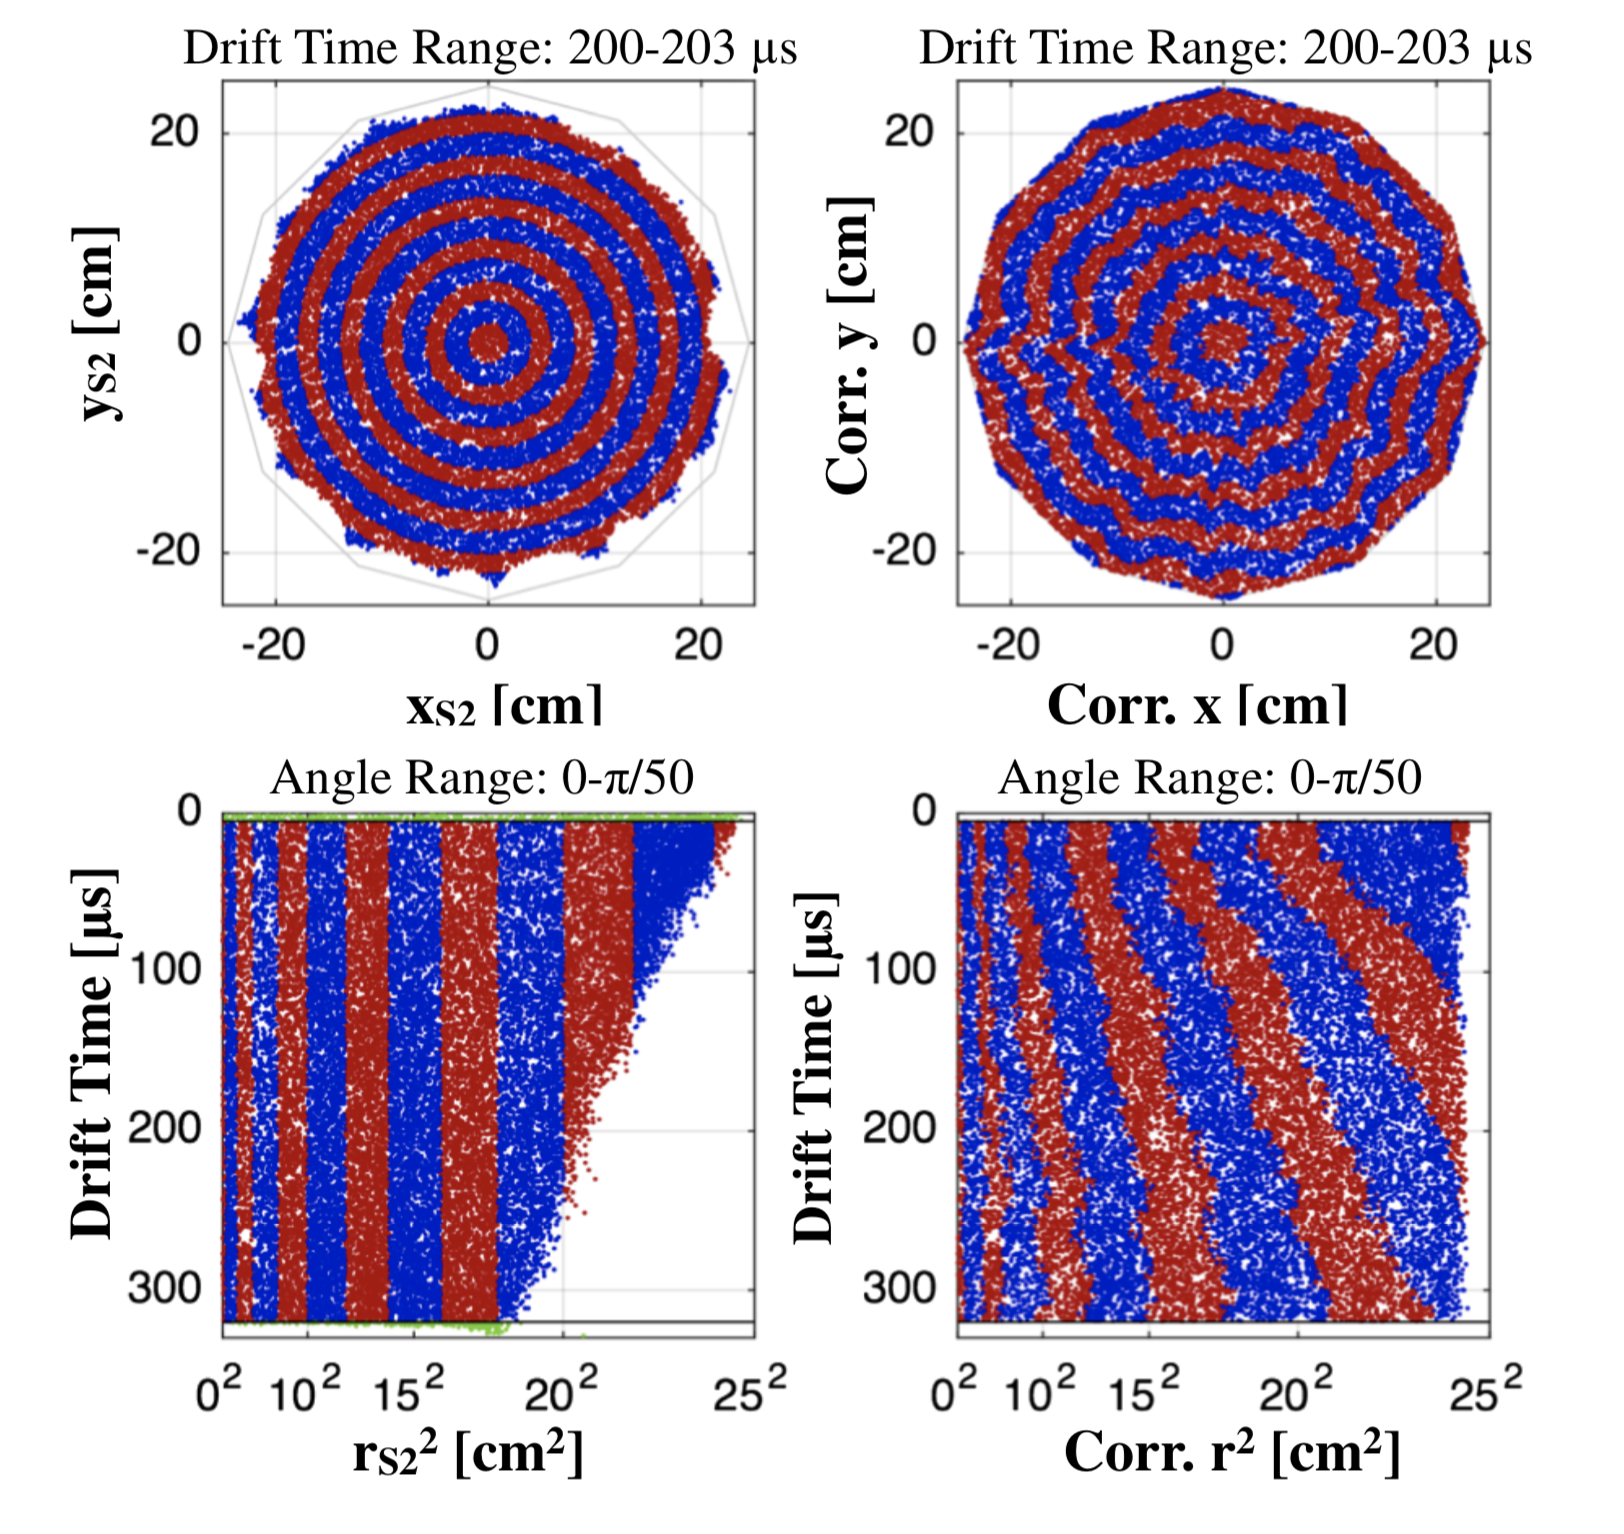
\includegraphics[width=.8\textwidth]{figures/lux/kr_pos2.png}
\caption{ The effect of radial position mapping between S2 coordinates (left) and real coordinates (right). The top panels show a thin horizontal slice of the detector and the bottom panels show a thin vertical slide. The red and blue colors are to made the effect of the mapping visible. Note that squared radius in the bottom panels exaggerates the scale of the effect. Figure from \cite{LUXKr} }
\label{fig:kr_pos2}
\end{center}
\end{figure}

In addition to the small radial dependence, the electric fields illustrated in Figure~\ref{fig:kr_pos1} also vary in magnitude. The two decays of $^{83m}$Kr can be leveraged to directly probe the magnitude of the field, as they exhibit different field dependence (recall from Chapter~\ref{sec:energy_reconstruction} that signal yields depend on applied field and particle energy). The ratio of S1a to S1b increases with field, and provides a measure of the spatial dependence of the magnitude of the electric field. A highly variant electric field would affect recombination, and cause different light and charge yields at different positions in the detector, in turn affecting sensitivity. The fields measured via this method in Run03 were found to only cause corrections on the order of a percent and so no field-dependent corrections were applied \cite{LUXKr}. However, in Run04 the ratio technique was of central importance (see \cite{LUXCombinedExposure} \cite{LUXFields} \cite{LUXKr} for more detail). The result of the ratio method for measuring electric field magnitude is shown in Figure~\ref{fig:kr_3} for Run03 fields.

\begin{figure}[htbp]
\begin{center}
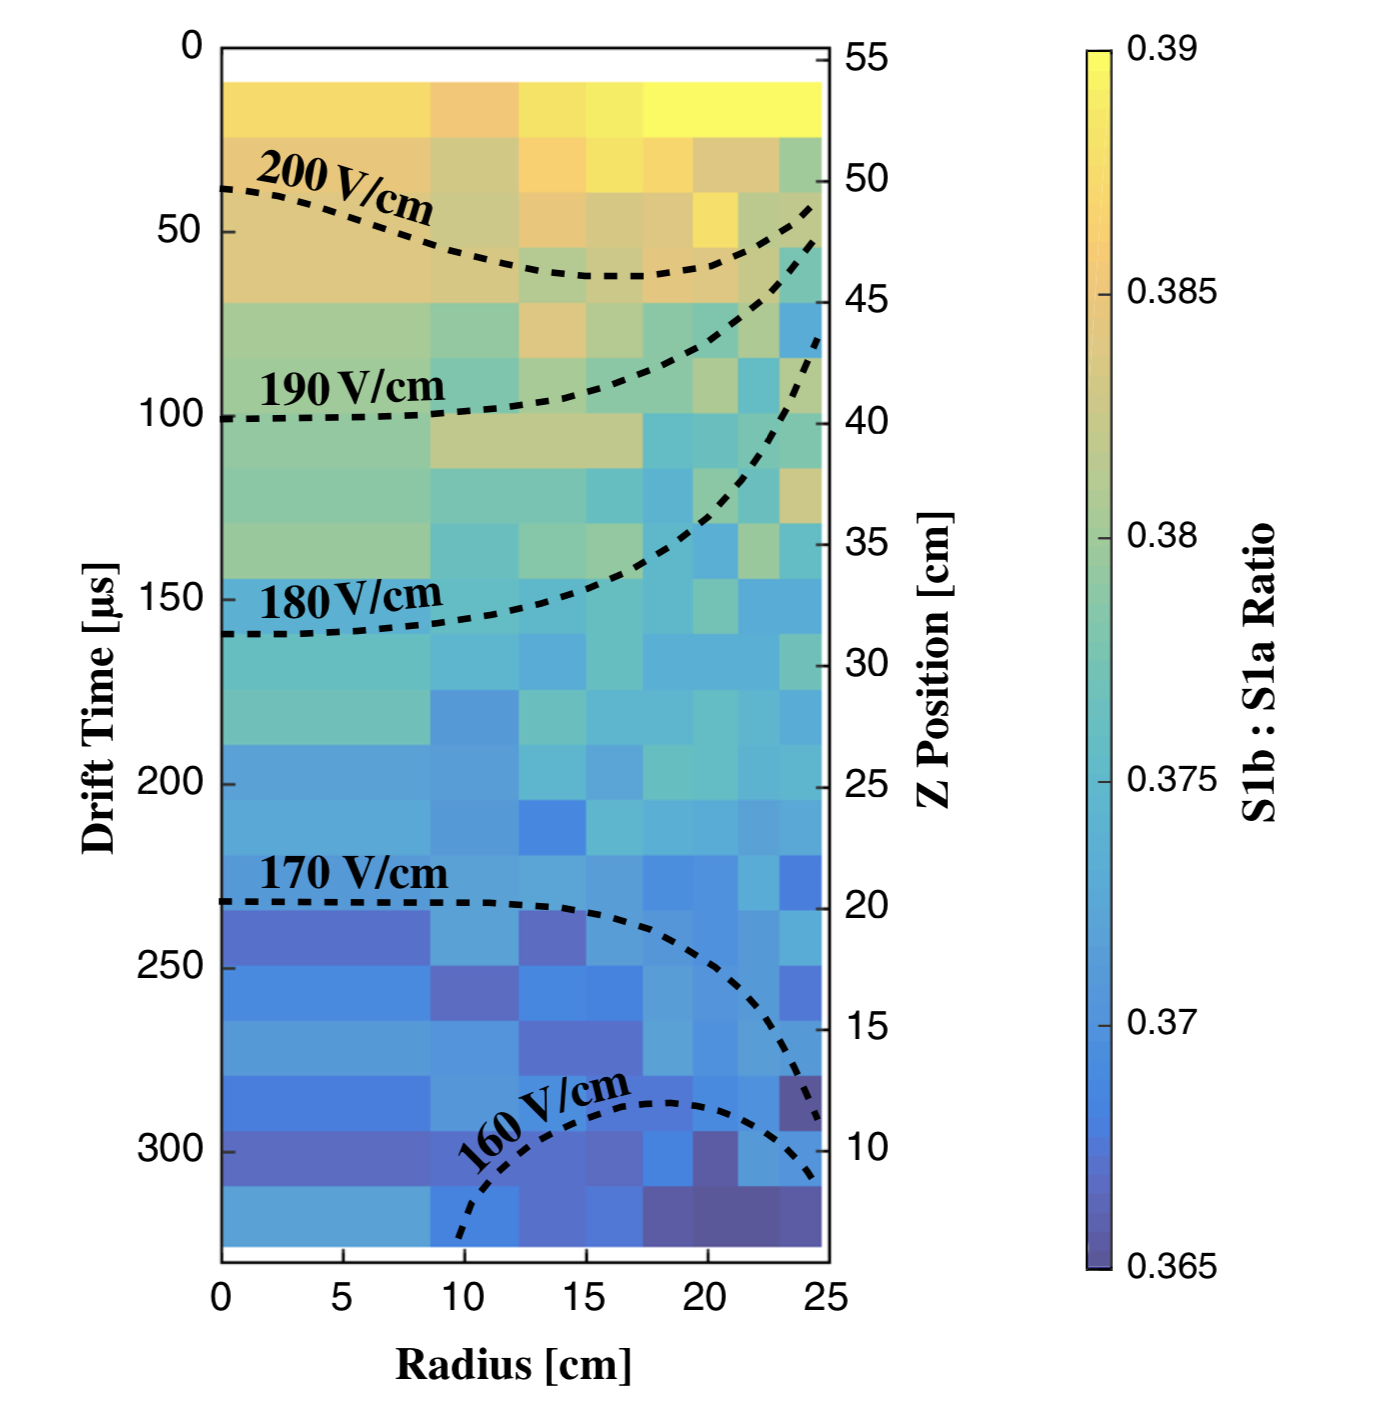
\includegraphics[width=0.69\textwidth]{figures/lux/kr_3.png}
\caption{Field map of Run03 produced by $^{83m}$Kr S1a:S1b ratio. Because only a fraction of $^{83m}$Kr produce separate S1a and S1b, the bins are large to accomidate reduced statistics. Figure from \cite{LUXKr} }
\label{fig:kr_3}
\end{center}
\end{figure}

\FloatBarrier
\subsection{Tritium Beta Decay: Calibration of the ER Band and Yields}
In order to calibrate the \ac{ER} band of \ac{LUX} a $\beta$ source in the \ac{WIMP} energy range (1 to 8~keV$_{ee}$) was needed. \ac{LUX} used a gaseous tritiated methane (CH$_{3}$T) source to deliver tritium uniformly into the active volume. Tritiated methane was chosen over the molecular tritium (T$_{2}$) because it does not adsorb onto surfaces like the smaller T$_{2}$ molecule and it does not interfere with charge transport in \ac{LXe} \cite{LUXTritium}. Tritium has a Q-value of 18.6~keV, but the spectrum peaks at 2.5~keV, with 64.2\% of the decays occurring in the \ac{WIMP} search energy range \cite{LUXTritium}. The half-life of tritium is 12.3~years, so efficient removal was essential. \ac{LUX} demonstrated that once deployed, CH$_{3}$T was removed with a 6~hour time constant, returning the detector back to acceptable \ac{WIMP} search rates. CH$_{3}$T was shipped to site in a bottle, mixed with purified xenon and released into the circulation system after the getter, to be swept into the inner volume. 

The tritium energy spectrum from data is shown with the theoretical energy spectrum convoluted with the detector energy resolution in Figure~\ref{fig:tritium1} (left). The ratio of the the two is shown in Figure~\ref{fig:tritium1} (right), demonstrating a 50\% effective energy threshold for \ac{ER} events at 1.24 $\pm$ 0.026~keV. The agreement between data and theory shows powerful support for the energy model E = W (S1/g$_{1}$ + S1/g$_{2}$). 

\begin{figure}[htbp]
\begin{center}
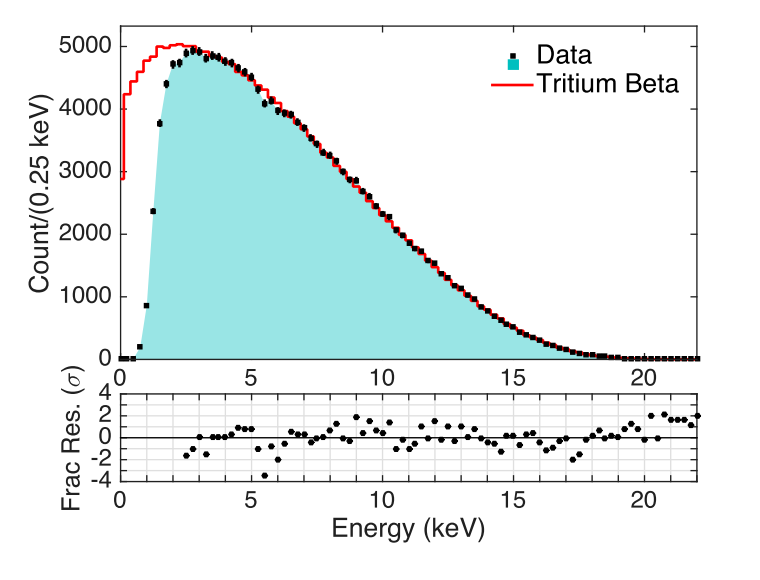
\includegraphics[width=\halffig]{figures/lux/lux_tritium1a.png}
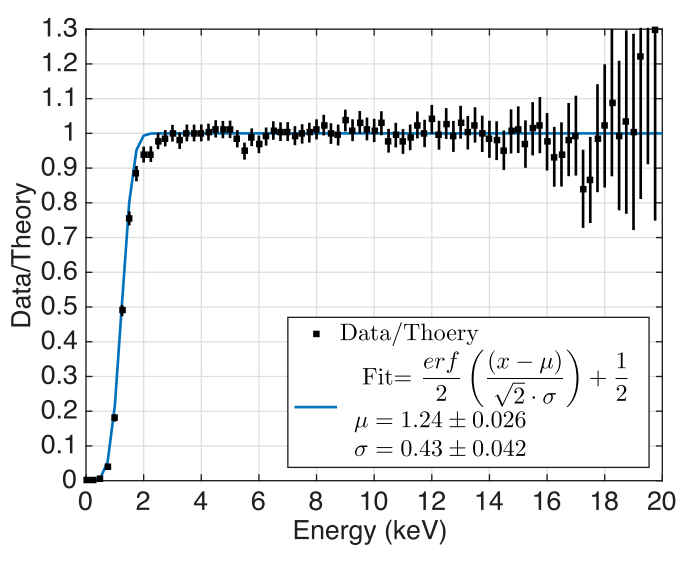
\includegraphics[width=\halffig]{figures/lux/lux_tritium1b.png}
\caption{ (left) Plot showing the theoretical tritium beta spectrum with the spectrum obtained from data, and residuals. (right) The ratio of data to theory convoluted with the detector energy resolution. Figure from \cite{LUXTritium}.}
\label{fig:tritium1}
\end{center}
\end{figure}

Tritium was also used to measure the light and charge yields over a wide energy range. Figure~\ref{fig:tritium3} (left) shows the detected number of quanta, $n_{\gamma}$ and $n_{e}$. Recall that is this is not necessarily the number of initial quanta $n_{ex}$ and $n_{ion}$ that are produced, as some number of $n_{ion}$ undergo recombination to produce additional scintillation photons.  Figure~\ref{fig:tritium3} (right) shows the effect that event energy has on recombination. For \ac{ER} events $n_{ex} / n_{ion} = 0.2$ is assumed to be constant \cite{LUX:YieldsAndRecombination}, but the observed ratio $n_{\gamma} / n_{e}$ is clearly energy dependent.

\begin{figure}[htbp]
\begin{center}
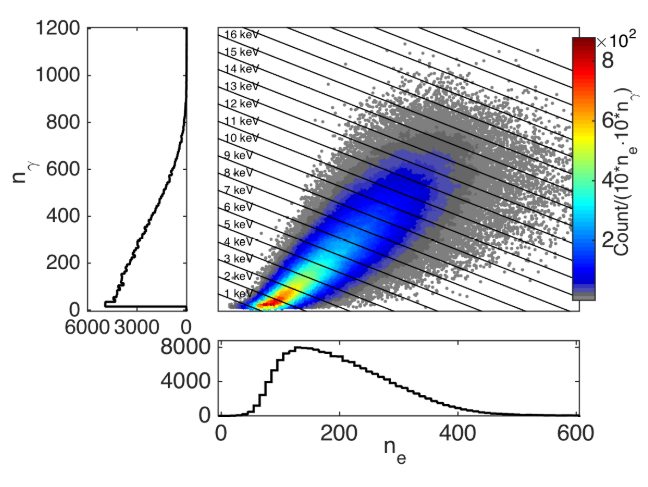
\includegraphics[width=\halffig]{figures/lux/lux_tritium3a.png}
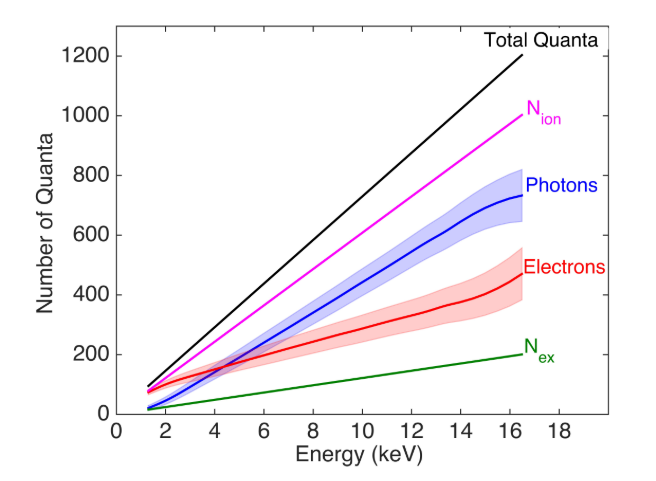
\includegraphics[width=\halffig]{figures/lux/lux_tritium3b.png}
\caption{ (left) The measured quanta yields shown with lines of equal energy. (right) A plot depicting the expected initial quanta yields, $N_{ion}$ and $N_{ex}$, compared with the measured yield of photons and electrons. The difference is caused by the energy dependence of recombination. Figure from \cite{LUXTritium}.}
\label{fig:tritium3}
\end{center}
\end{figure}

Lastly, tritium was used to construct the \ac{ER} band (Figure~\ref{fig:tritium2} (left)), which is necessary for \ac{WIMP} search. The width of the \ac{ER} band is of significant interest, as it determines the nuclear recoil discrimination of the detector. The number of \ac{ER} events from the tritium calibration that occur below the nuclear recoil band mean is known as leakage fraction, $f$, and is shown as a function of energy in Figure~\ref{fig:tritium2} (right). The average \ac{ER} discrimination efficiency ($1-f$) for Run03 was 99.81\% $\pm$ 0.02\%(stat) $\pm$ 0.1\%(sys), where the systematic error comes from the error on $g_{1}$ and $g_{2}$. This measurement of discrimination efficiency relies on knowing the mean and width of the \ac{NR} band, which is discussed in the next section.

\begin{figure}[htbp]
\begin{center}
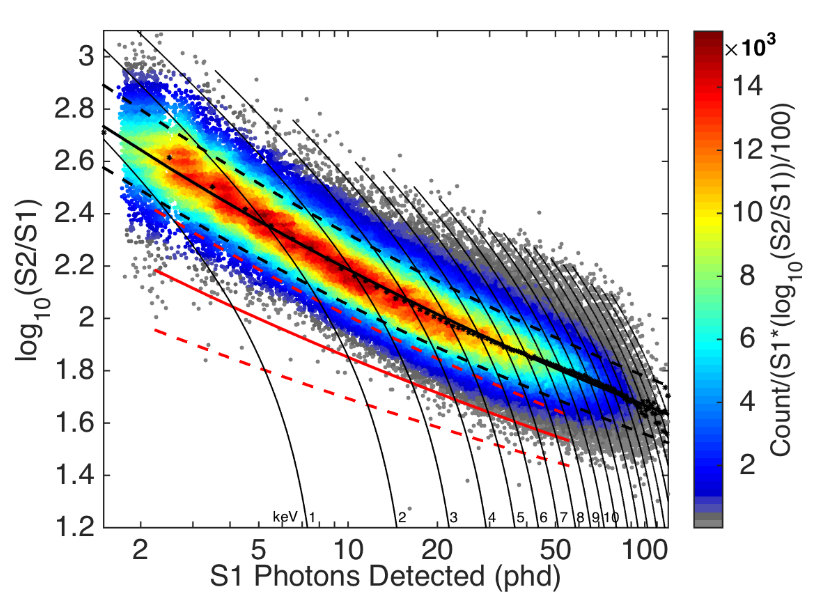
\includegraphics[width=\halffig]{figures/lux/lux_tritium2a.png}
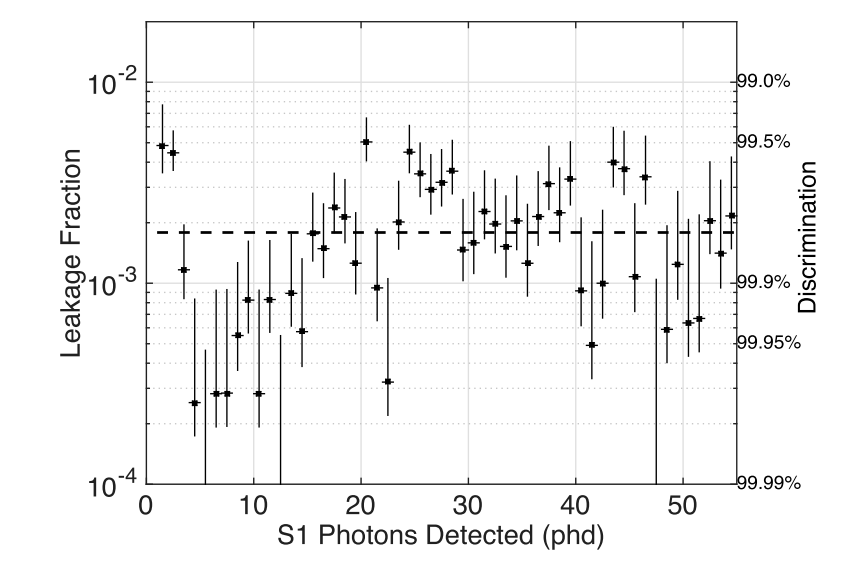
\includegraphics[width=\halffig]{figures/lux/lux_tritium2b.png}
\caption{ (left) The \acs{ER} band for in \acs{WIMP} search energy range obtained from the tritium calibration. (right) Leakage fraction of \acs{ER} events below the \acs{NR} mean in the \acs{WIMP} search energy range. Knowledge of the \acs{NR} band comes from the \acs{DD} calibration detailed in Section~\ref{sec:DD}. Figure from \cite{LUXTritium}.}
\label{fig:tritium2}
\end{center}
\end{figure}

\subsection{Deuterium-Deuterium (DD) Neutrons: Calibration of the NR Band and Yields}
\label{sec:DD}
Low energy neutrons from a \ac{DD} generator were used to calibrate the \ac{NR} response and signal yields for \ac{LUX} in the \ac{WIMP} search energy range. A photo and diagram of the calibration scheme are shown in Figure~\ref{fig:dd_gen}. Following Run03, \ac{LUX} employed the \ac{DD} generator to deliver a collimated beam of 2.45~MeV neutrons into the \ac{TPC}. As Figure~\ref{fig:dd_gen} shows, the generator was positioned outside the water tank, but when aligned with the neutron conduit (a \ac{PVC} tube of air), deposited neutrons into the \ac{LXe} space. The \ac{DD} calibration leverages known kinematics of neutron scattering, the known incoming neutron energies, and the known detector gains $g_{1}$ and $g_{2}$ to develop a complete characterization of low-engergy \ac{NR} in \ac{LUX}. The method is summarized here, but details are available in \cite{LUXDD}.

\begin{figure}[htbp]
\begin{center}
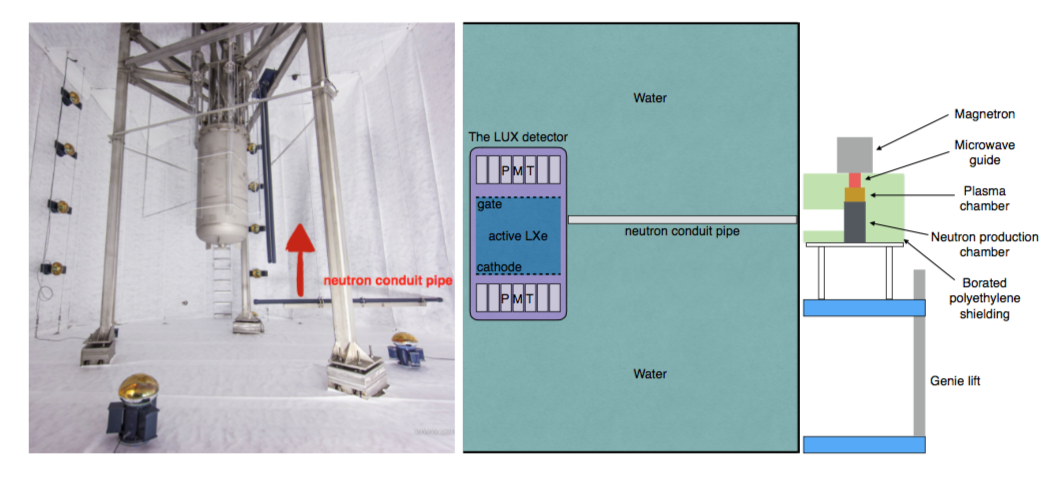
\includegraphics[width=\textwidth]{figures/lux/lux_ddgenerator.png}
\caption{(left) Photo of the water tank interior showing the neutron conduit, which is raised during \acs{DD} calibration. (right) Diagram of the \acs{DD} generator and water tank neutron conduit during \acs{DD} operation. Figure courtesy of E. Pease.}
\label{fig:dd_gen}
\end{center}
\end{figure}

First, charge yield was derived from a population of multiscatter events: those with one S1 (the S1s are merged due to simultaneous collection of S1s) and two S2s (separated in space and z-position/drift time). Neutron scattering kinematics allow for the reconstruction of energy at the first scatter site, so the unknown first S1 is not needed to ascertain the energy deposition. The charge yield is then obtained from the first S2 and the energy of the first scatter from kinematics. 

Once the charge yield was obtained, a population of single scatter events was collected: one S1 and one S2. These events were from neutrons that scattered once the detector, and then exited. Here, the second scatter is not available to kinematically reconstruct energy, so instead the charge yield is employed to infer the energy of the single scatter. The light yield is then obtained from the S1 and the energy deposition inferred from charge yield. 

It should be noted that though the \ac{DD} generator produced monoenergetic neutrons of initial energy $E_{i}$, the energy deposited $E_{d}$ by a neutron scatter is

\begin{equation}
E_{d} = E_{i} \frac{m_{n} M_{Xe}}{m_{n} + M_{Xe}} sin^{2}\theta_{CM}
\end{equation}

Where $m_{n}$ in the neutron mass, $M_{Xe}$ is the xenon mass, and $\theta_{CM}$ is the scattering angle relative to the neutron conduit in the center of mass frame. The deposited energy, $E_{d}$ then covers a range of energies, allowing for calibration of the \ac{NR} band and yields over a range of energies. After determination of the light yield, the single scatter events were used to construct the \ac{NR} band in Figure~\ref{fig:lux_nrband}.

\begin{figure}[htbp]
\begin{center}
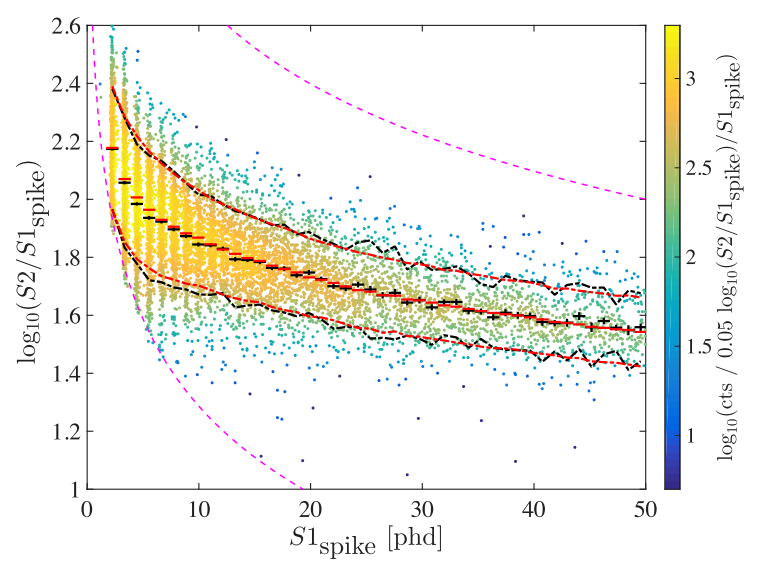
\includegraphics[width=\textwidth]{figures/lux/lux_nrband.png}
\caption{Calibration showing the \acs{NR} band mean and width from the \acs{DD} calibration. The x-axis is S1$_{spike}$, for which candidate single photons (``spikes'') are identified and tallied in sparse waveforms. This can be a more accurate photon count for low energies and is preferred here to the usual integrated waveform method (see \cite{LUXReanalysis} for more information). The black data points are the Gaussian fit centroid values for each S1spike bin. The red data points are corresponding Gaussian fit mean value for the simulated nuclear recoil band produced using the model described in Sec. VII. The black and red dot-dashed lines indicate the 90\% one-sided limits from data and simulation, respectively. The magenta dashed lines indicate the lower and upper S2 thresholds applied to the \acs{WIMP} search. Error bars are statistical only. Figure from \cite{LUXDD}.}
\label{fig:lux_nrband}
\end{center}
\end{figure}



\FloatBarrier
\subsection{Energy Resolution and Signal Yields Outside the WIMP Search Range}
\label{sec:highenergyyeilds}
The extensive calibration programs outlined above focus on the \ac{WIMP} search energy range of 1-8~keV$_{ee}$ ($\sim$8-33~keV$_{nr}$). The \ac{LUX} detector is optimized for low-energy sensitivity, and so this is where most of the calibration effort is focused. However, \ac{LUX} carried out a detailed study of the energy resolution and signal yields in an energy range complementary to the \ac{WIMP} search range. The study is presented in \cite{LUX:YieldsAndRecombination}, and utilized the rich spectrum of radioactive decays present during Run03 (see Figure~\ref{fig:luxspectrum}), many of which were also used in the Doke plot analysis discussed above. The spectrum continued above what is shown in Figure~\ref{fig:luxspectrum}, but the peaks are increasingly difficult to isolate from the Compton scatter continuum and so were not used in the study. In addition to the peaks in the high energy \ac{ER} spectrum, the external $^{137}$Cs calibration source with energy 662~keV was used in the study. This source is the highest energy calibration source used in \ac{LUX}; the detector is not extensively characterized above 662~keV. 

\begin{figure}[htbp]
\begin{center}
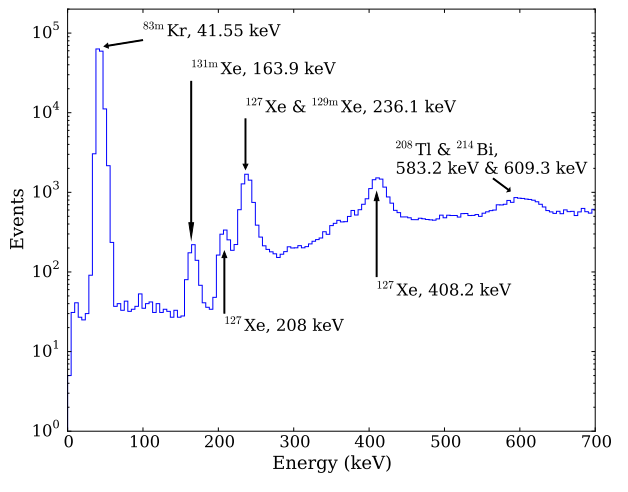
\includegraphics[width=\textwidth]{figures/lux/luxspectrum.png}
\caption{Single-scatter events identified in the \acs{LUX} 2013 \acs{WIMP}-search data. The labels indicate the source isotopes and their energies. In addition to single scatters, some of these isotopes have other decay modes that can produce multiple scatters. Figure from \cite{LUX:YieldsAndRecombination}.}
\label{fig:luxspectrum}
\end{center}
\end{figure}

The signal yields of these high energy lines were found to be in consistent agreement with \ac{NEST} \cite{LUX:YieldsAndRecombination}. \ac{NEST} is a widely used simulation package for modeling noble element scintillation; more information can be found about \ac{NEST} in \cite{Szydagis2011}. The agreement between \ac{LUX} and \ac{NEST} demonstrates that \ac{LUX} detector performance is understood in a wide range of energies. 

The energy resolution of these high energy lines was also studied. In general, as energy increases, the resolution is expected to increase. This is because as more energy is deposited, more quanta are generated, and therefore the same detector can collect more signal. The expected behavior of the energy resolution has, naively, a underlying Poisson nature: $\sigma / \mu \sim \sqrt{E}/E$. In reality, there are restrictions on the number of ways in which an atom can be ionized so the energy resolution is not purely statistical, but better. The number of quanta generated cannot feely fluctuate, but depends on the stopping material, and is characterized by a factor called the Fano factor \cite{Fano1947} \cite{Aprile2010}. The ultimate energy resolution of a \ac{LXe} detector is given by \cite{Aprile2010}: 

\begin{equation}
\frac{\Delta E}{E} = 2.35 \frac{\sqrt{F W_{LXe} E} }{E} 
\end{equation}

Where $\Delta E$ is the full width at half maximum of a fit to the peak, $F$ is the Fano factor in \ac{LXe}, and $W_{LXe}$ is the W-value. The energy resolution of \ac{LUX}, measured as $\sigma / \mu$, is presented in Figure~\ref{fig:energy_resolution}. The empirical function $a / \sqrt{E} $ is fit to the results, yielding $a = (0.33 \pm 0.01$~keV$^{1/2}$). The energy resolution is poorer than expected at high energies, and this is due to a series of systematics that are discussed in depth in \cite{LUX:YieldsAndRecombination}. In summary, the resolution at high energy energies is limited by \ac{DAQ} saturation, \ac{PMT} saturation, and delayed electron noise. The latter two issues and their effects on energy resolution are discussed in depth in Chapter~\ref{ch:etrains}. Here we just note that with large enough energy deposits, \ac{PMT} response becomes non-linear, and delayed electron noise contributes spurious area to pulses. \ac{DAQ} saturation refers to an incoming \ac{PMT} voltage signal reaching the maximum of the \ac{ADC} range of the Struck digitizers. A method to ``bypass'' \ac{PMT} saturation is used in \ac{LUX}: \ac{PMT} saturation from high energy events is primarily of concern in the top array due to the proximity of the S2 light and the \ac{PMT}s. Instead, the bottom \ac{PMT} array only can be used in energy reconstruction. This method has been used in \ac{LUX} to aid in reconstructing the energies to correctly identify various high energy background populations.

\begin{figure}[htbp]
\begin{center}
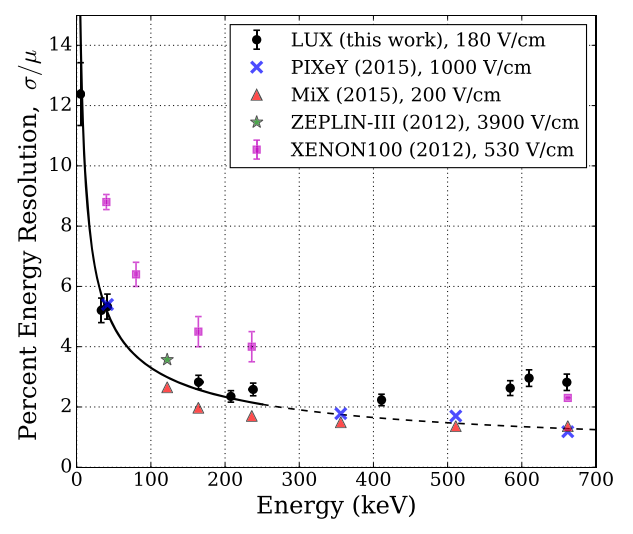
\includegraphics[width=\textwidth]{figures/lux/energy_resolution.png}
\caption{The measured energy resolution at known energy peaks in the LUX ER backgrounds. The detector is optimized for low-energy sensitivity, and variable amounts of PMT saturation and single-electron contributions affect S2 pulses and hamper the energy resolution at high energy. An empirical fit $a / \sqrt{E} $ is applied. Figure from \cite{LUX:YieldsAndRecombination}.}
\label{fig:energy_resolution}
\end{center}
\end{figure}

Some of the expected \ac{LIP} signals discussed in the next chapter can deposit large amounts of energy; the analysis benefits from the study of yields and detector response presented in \ac{LUX:YieldsAndRecombination}.
%The systematics at play in high energy interactions were studied in depth for the analysis presented in \cite{LUX:YieldsAndRecombination},

%The highest energy calibration source, $^{137}$Cs with energy 662~keV, exhibits a small amount of \ac{PMT} saturation in the top \ac{PMT} array due to the large number of S2 photons generated in close proximity to the \ac{PMT}s. \ac{PMT} saturation is discussed in more detail in Chapter~\ref{sec:testbed_measurement_challenges}, but here we just note that with large enough energy deposits, \ac{PMT} response becomes non-linear. This means that after a certain energy, we expect the formula $E = W (S1/g_{1} + S2/g_{2}) $ to fail, and we lose the accuracy and resolution of energy reconstruction that we enjoy in the \ac{WIMP} search range. Since \ac{PMT} saturation from high energy events is primarily of concern in the top array due to the proximity of the S2 light and the \ac{PMT}s, only the bottom \ac{PMT} array can be used in energy reconstruction. This method has been used in \ac{LUX} to aid in reconstructing the energies to correctly identify various high energy background populations.

%The systematics at play in high energy interactions were studied in depth for the analysis presented in \cite{LUX:YieldsAndRecombination}. 


\FloatBarrier
\subsection{Significance of LUX Calibrations}
Although this thesis is concerned mainly with a search for \ac{LIP}s, it should be noted that the extensive \ac{LUX} calibrations allowed for excellent understanding of the detector, resulting in a world-leading \ac{WIMP} limit. In particular, the \ac{DD} calibration (carried out after Run03) yielded a much better understanding of the \ac{NR} band and yields, and therefore detector thresholds, than the initial AmBe neutron calibration which was carried out in the early days of \ac{LUX}. The power of the \ac{DD} calibration can be seen in the difference between the first \ac{LUX} result \cite{LUXFirstResults} and the Run03 re-analysis \cite{LUXReanalysis} shown in Figure~\ref{fig:lux_reanalysis}. In particular, improved knowledge of the scintillation yields allowed a re-analysis threshold down to 1.1~keV$_{nr}$ where the initial \ac{WIMP} search adopted the more conservative threshold of 3.0~keV$_{nr}$. This improvement allowed \ac{LUX} to exclude new spin-independent parameter space below a \ac{WIMP} mass of 10~GeV. 


\begin{figure}[htbp]
\begin{center}
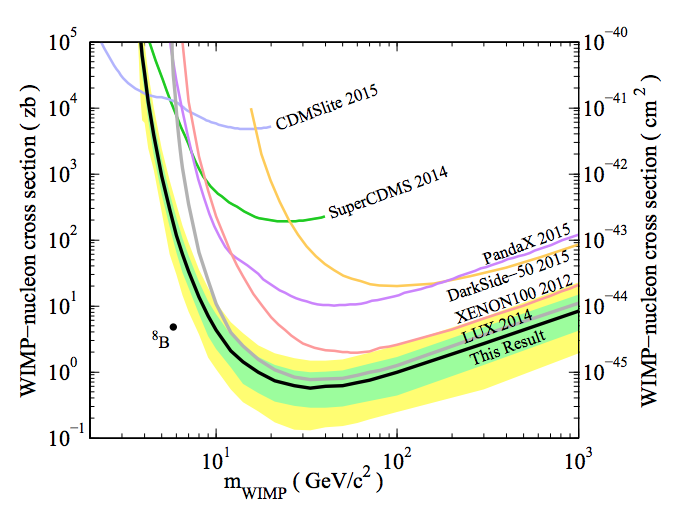
\includegraphics[width=\textwidth]{figures/lux/lux_reanalysis.png}
\caption{Improved spin-independent \acs{WIMP} limit of the Run03 exposure following the \acs{DD} calibration of \acs{LUX}. The first Run03 limit is the gray line labelled LUX~2014, the improved Run03 observed limit is the black line labelled This Result.  Figure from \cite{LUXReanalysis}.}
\label{fig:lux_reanalysis}
\end{center}
\end{figure}

Above the \ac{WIMP} search energy range, the analysis presented in \cite{LUX:YieldsAndRecombination}, and discussed above in Section~\ref{sec:highenergyyeilds}, was used to further improve and test knowledge of the xenon microphysics responsible for signal generation. Understanding of the \ac{LUX} detector response was extended over a wide range of energies.


%*****************************************
%*****************************************
%*****************************************
%*****************************************
%*****************************************
